\documentclass[11pt]{article}
%DIF LATEXDIFF DIFFERENCE FILE
%DIF DEL /tmp/main_old.tex   Thu Jul 16 09:38:23 2026
%DIF ADD main.tex            Thu Jul 16 09:35:34 2026

\usepackage{amsmath, amsthm, amssymb}
\usepackage[hidelinks]{hyperref}
\usepackage{geometry}
\geometry{margin=1in}
\usepackage{authblk}
\usepackage{graphicx}
\usepackage{booktabs}

\newtheorem{theorem}{Theorem}
\newtheorem{proposition}{Proposition}
\newtheorem{lemma}{Lemma}
\newtheorem{corollary}{Corollary}
\newtheorem{definition}{Definition}
\newtheorem{remark}{Remark}

\newcommand{\bfa}{\mathbf{a}}
\newcommand{\bfb}{\mathbf{b}}
\newcommand{\intro}{\mathrm{intro}}
\newcommand{\pC}{p_C}

\title{Introspection Dynamics with Mutation in Additive Games}
\author[1]{Harry Foster}
\author[1,*]{Vince Knight}
\author[2]{Sebastian Krapohl}
\affil[1]{School of Mathematics, Cardiff University}
\affil[2]{Faculty of Social and Behavioural Sciences, University of Amsterdam}
\affil[*]{Corresponding author: \texttt{knightva@cardiff.ac.uk}}
\date{\today}
%DIF PREAMBLE EXTENSION ADDED BY LATEXDIFF
%DIF UNDERLINE PREAMBLE %DIF PREAMBLE
\RequirePackage[normalem]{ulem} %DIF PREAMBLE
\RequirePackage{color}\definecolor{RED}{rgb}{1,0,0}\definecolor{BLUE}{rgb}{0,0,1} %DIF PREAMBLE
\providecommand{\DIFaddtex}[1]{{\protect\color{blue}\uwave{#1}}} %DIF PREAMBLE
\providecommand{\DIFdeltex}[1]{{\protect\color{red}\sout{#1}}}                      %DIF PREAMBLE
%DIF SAFE PREAMBLE %DIF PREAMBLE
\providecommand{\DIFaddbegin}{} %DIF PREAMBLE
\providecommand{\DIFaddend}{} %DIF PREAMBLE
\providecommand{\DIFdelbegin}{} %DIF PREAMBLE
\providecommand{\DIFdelend}{} %DIF PREAMBLE
\providecommand{\DIFmodbegin}{} %DIF PREAMBLE
\providecommand{\DIFmodend}{} %DIF PREAMBLE
%DIF FLOATSAFE PREAMBLE %DIF PREAMBLE
\providecommand{\DIFaddFL}[1]{\DIFadd{#1}} %DIF PREAMBLE
\providecommand{\DIFdelFL}[1]{\DIFdel{#1}} %DIF PREAMBLE
\providecommand{\DIFaddbeginFL}{} %DIF PREAMBLE
\providecommand{\DIFaddendFL}{} %DIF PREAMBLE
\providecommand{\DIFdelbeginFL}{} %DIF PREAMBLE
\providecommand{\DIFdelendFL}{} %DIF PREAMBLE
%DIF HYPERREF PREAMBLE %DIF PREAMBLE
\providecommand{\DIFadd}[1]{\texorpdfstring{\DIFaddtex{#1}}{#1}} %DIF PREAMBLE
\providecommand{\DIFdel}[1]{\texorpdfstring{\DIFdeltex{#1}}{}} %DIF PREAMBLE
\newcommand{\DIFscaledelfig}{0.5}
%DIF HIGHLIGHTGRAPHICS PREAMBLE %DIF PREAMBLE
\RequirePackage{settobox} %DIF PREAMBLE
\RequirePackage{letltxmacro} %DIF PREAMBLE
\newsavebox{\DIFdelgraphicsbox} %DIF PREAMBLE
\newlength{\DIFdelgraphicswidth} %DIF PREAMBLE
\newlength{\DIFdelgraphicsheight} %DIF PREAMBLE
% store original definition of \includegraphics %DIF PREAMBLE
\LetLtxMacro{\DIFOincludegraphics}{\includegraphics} %DIF PREAMBLE
\newcommand{\DIFaddincludegraphics}[2][]{{\color{blue}\fbox{\DIFOincludegraphics[#1]{#2}}}} %DIF PREAMBLE
\newcommand{\DIFdelincludegraphics}[2][]{% %DIF PREAMBLE
\sbox{\DIFdelgraphicsbox}{\DIFOincludegraphics[#1]{#2}}% %DIF PREAMBLE
\settoboxwidth{\DIFdelgraphicswidth}{\DIFdelgraphicsbox} %DIF PREAMBLE
\settoboxtotalheight{\DIFdelgraphicsheight}{\DIFdelgraphicsbox} %DIF PREAMBLE
\scalebox{\DIFscaledelfig}{% %DIF PREAMBLE
\parbox[b]{\DIFdelgraphicswidth}{\usebox{\DIFdelgraphicsbox}\\[-\baselineskip] \rule{\DIFdelgraphicswidth}{0em}}\llap{\resizebox{\DIFdelgraphicswidth}{\DIFdelgraphicsheight}{% %DIF PREAMBLE
\setlength{\unitlength}{\DIFdelgraphicswidth}% %DIF PREAMBLE
\begin{picture}(1,1)% %DIF PREAMBLE
\thicklines\linethickness{2pt} %DIF PREAMBLE
{\color[rgb]{1,0,0}\put(0,0){\framebox(1,1){}}}% %DIF PREAMBLE
{\color[rgb]{1,0,0}\put(0,0){\line( 1,1){1}}}% %DIF PREAMBLE
{\color[rgb]{1,0,0}\put(0,1){\line(1,-1){1}}}% %DIF PREAMBLE
\end{picture}% %DIF PREAMBLE
}\hspace*{3pt}}} %DIF PREAMBLE
} %DIF PREAMBLE
\LetLtxMacro{\DIFOaddbegin}{\DIFaddbegin} %DIF PREAMBLE
\LetLtxMacro{\DIFOaddend}{\DIFaddend} %DIF PREAMBLE
\LetLtxMacro{\DIFOdelbegin}{\DIFdelbegin} %DIF PREAMBLE
\LetLtxMacro{\DIFOdelend}{\DIFdelend} %DIF PREAMBLE
\DeclareRobustCommand{\DIFaddbegin}{\DIFOaddbegin \let\includegraphics\DIFaddincludegraphics} %DIF PREAMBLE
\DeclareRobustCommand{\DIFaddend}{\DIFOaddend \let\includegraphics\DIFOincludegraphics} %DIF PREAMBLE
\DeclareRobustCommand{\DIFdelbegin}{\DIFOdelbegin \let\includegraphics\DIFdelincludegraphics} %DIF PREAMBLE
\DeclareRobustCommand{\DIFdelend}{\DIFOaddend \let\includegraphics\DIFOincludegraphics} %DIF PREAMBLE
\LetLtxMacro{\DIFOaddbeginFL}{\DIFaddbeginFL} %DIF PREAMBLE
\LetLtxMacro{\DIFOaddendFL}{\DIFaddendFL} %DIF PREAMBLE
\LetLtxMacro{\DIFOdelbeginFL}{\DIFdelbeginFL} %DIF PREAMBLE
\LetLtxMacro{\DIFOdelendFL}{\DIFdelendFL} %DIF PREAMBLE
\DeclareRobustCommand{\DIFaddbeginFL}{\DIFOaddbeginFL \let\includegraphics\DIFaddincludegraphics} %DIF PREAMBLE
\DeclareRobustCommand{\DIFaddendFL}{\DIFOaddendFL \let\includegraphics\DIFOincludegraphics} %DIF PREAMBLE
\DeclareRobustCommand{\DIFdelbeginFL}{\DIFOdelbeginFL \let\includegraphics\DIFdelincludegraphics} %DIF PREAMBLE
\DeclareRobustCommand{\DIFdelendFL}{\DIFOaddendFL \let\includegraphics\DIFOincludegraphics} %DIF PREAMBLE
%DIF COLORLISTINGS PREAMBLE %DIF PREAMBLE
\RequirePackage{listings} %DIF PREAMBLE
\RequirePackage{color} %DIF PREAMBLE
\lstdefinelanguage{DIFcode}{ %DIF PREAMBLE
%DIF DIFCODE_UNDERLINE %DIF PREAMBLE
  moredelim=[il][\color{red}\sout]{\%DIF\ <\ }, %DIF PREAMBLE
  moredelim=[il][\color{blue}\uwave]{\%DIF\ >\ } %DIF PREAMBLE
} %DIF PREAMBLE
\lstdefinestyle{DIFverbatimstyle}{ %DIF PREAMBLE
	language=DIFcode, %DIF PREAMBLE
	basicstyle=\ttfamily, %DIF PREAMBLE
	columns=fullflexible, %DIF PREAMBLE
	keepspaces=true %DIF PREAMBLE
} %DIF PREAMBLE
\lstnewenvironment{DIFverbatim}{\lstset{style=DIFverbatimstyle}}{} %DIF PREAMBLE
\lstnewenvironment{DIFverbatim*}{\lstset{style=DIFverbatimstyle,showspaces=true}}{} %DIF PREAMBLE
%DIF END PREAMBLE EXTENSION ADDED BY LATEXDIFF

\begin{document}

\maketitle

\begin{abstract}
Cooperation in heterogeneous groups, where individuals differ in resources,
productivity, and behavioural responsiveness, underpins collective action
across social and biological systems. Introspection dynamics \DIFdelbegin \DIFdel{, in which each }\DIFdelend \DIFaddbegin \DIFadd{is a learning
rule suited to such asymmetric settings: at each time step a randomly
selected }\DIFaddend player compares their \DIFdelbegin \DIFdel{payoff to their payoff under the alternative action}\DIFdelend \DIFaddbegin \DIFadd{current payoff to the payoff an alternative
action would have given, and switches with a probability increasing in the
difference. We extend introspection dynamics to include }\emph{\DIFadd{mutation}}\DIFadd{,
where a selected player adopts an action with payoff-independent}\DIFaddend ,
\DIFdelbegin \DIFdel{provides a natural learning rule for such asymmetric settings. }\DIFdelend \DIFaddbegin \DIFadd{player-specific probabilities, together with player-specific selection
intensities. From the extended dynamics we rederive and generalise the
results of }\DIFaddend Couto and Pal \DIFdelbegin \DIFdel{showed that }\DIFdelend for \emph{additive} games, those in which the
payoff difference a player evaluates when considering a switch is
independent of the other players' actions\DIFdelbegin \DIFdel{, }\DIFdelend \DIFaddbegin \DIFadd{: }\DIFaddend the stationary distribution
\DIFdelbegin \DIFdel{of introspection dynamics is }\DIFdelend \DIFaddbegin \DIFadd{remains }\DIFaddend a product measure\DIFdelbegin \DIFdel{. We extend this result to introspection dynamics with
}\emph{\DIFdel{mutation}}%DIFAUXCMD
\DIFdel{, where a selected playerswitches to a random action with some
probability independent of payoffs}\DIFdelend , \DIFdelbegin \DIFdel{and with player-specific selection
intensities. We show that the product structure is preserved, and we obtain
the explicit per-player }\DIFdelend \DIFaddbegin \DIFadd{and each player's long-run }\DIFaddend cooperation
probability \DIFdelbegin \DIFdel{\(p_i=\phi_i(\delta_i)(1-\mu_{i0}-\mu_{i1})+\mu_{i0}\)}\DIFdelend \DIFaddbegin \DIFadd{has an explicit form in terms of their own payoffs, selection
intensity, and mutation probabilities
alone}\DIFaddend . We consider the heterogeneous public goods game, where \(N\)
players may differ in their contributions\DIFdelbegin \DIFdel{\(\alpha_i\)}\DIFdelend , public goods multipliers \(r_i\),
and selection intensities \(\beta_i\); the long-run cooperation probability
admits \DIFdelbegin \DIFdel{the closed form }\[
  \DIFdel{\pC = \frac{1}{N}\sum_{i=1}^{N}
        \left[\frac{1-\mu_{i0}-\mu_{i1}}{1+e^{\,\beta_i\alpha_i(1-r_i/N)}}+\mu_{i0}\right].
}\]%DIFAUXCMD
\DIFdelend \DIFaddbegin \DIFadd{a closed form with \(N\) terms rather than \(2^N\).
}\DIFaddend Several structural consequences follow: a player-specific cooperation threshold at
\(r_i = N\) under symmetric mutation, a neutral-drift regime in which cooperation is
governed entirely by mutation bias, and a mutation-selection balance in which aggregate
cooperation is affine in the mutation rate, interpolating between \DIFdelbegin \DIFdel{the selection-driven
level }\DIFdelend \DIFaddbegin \DIFadd{selection }\DIFaddend and
neutrality. Mutation also regularises the strong-selection limit
\DIFdelbegin \DIFdel{, so the
closed form holds as }\DIFdelend \(\beta_i\to\infty\), where the mutation-free dynamics degenerate.
\end{abstract}

\section{Introduction}

The public goods game is a canonical model of cooperation in evolutionary game theory:
players decide whether to contribute to a common resource, which is multiplied and
redistributed, creating a tension between individual incentive and collective
benefit~\cite{nowak2006five}. Classical analyses assume a homogeneous population, but
real groups are heterogeneous: players differ in their productivity, their
contributions,
and how sensitively they respond to payoff differences~\cite{hauser2019social}.

A natural learning rule for such settings is \emph{introspection dynamics}, introduced
in~\cite{couto2022introspection}: at each time step a player
compares their current payoff to the payoff they \emph{would have received} had they
played \DIFdelbegin \DIFdel{the }\DIFdelend \DIFaddbegin \DIFadd{an }\DIFaddend alternative action (keeping all other players fixed), and switches with a
probability governed by this difference. Because the comparison is
self-referential rather than imitative, introspection applies to arbitrary asymmetric
games where role-model imitation is unavailable or unnatural.

\DIFdelbegin \DIFdel{In~\mbox{%DIFAUXCMD
\cite{couto2023multiplayer} }\hskip0pt%DIFAUXCMD
}\DIFdelend \DIFaddbegin \DIFadd{Introspection dynamics is closely related to the logit-response dynamics
studied in economics~\mbox{%DIFAUXCMD
\cite{blume1993statistical,alosferrer2010logit}}\hskip0pt%DIFAUXCMD
, in
which revising
players choose actions with probabilities exponential in their payoffs; the
Fermi rule is the two-action logit choice. Asymmetric games have also been
approached through evolutionary dynamics directly, for example
in~\mbox{%DIFAUXCMD
\cite{mcavoy2015asymmetric}}\hskip0pt%DIFAUXCMD
. The introspection model
of~\mbox{%DIFAUXCMD
\cite{couto2022introspection,couto2023multiplayer}}\hskip0pt%DIFAUXCMD
, however, contains no
mutation: a selected player switches action solely according to the Fermi
rule. Mutation, the adoption of a random action independently of payoffs, is
a standard ingredient of evolutionary and learning
dynamics~\mbox{%DIFAUXCMD
\cite{fudenberg2006evolutionary} }\hskip0pt%DIFAUXCMD
that accounts for exploration,
error, and behavioural noise~\mbox{%DIFAUXCMD
\cite{traulsen2009exploration}}\hskip0pt%DIFAUXCMD
. In this paper
we extend introspection dynamics to include per-player, per-action mutation,
together with player-specific selection intensities \(\beta_i\) rather than
a single global value.
}

\DIFadd{From the extended dynamics we rederive, and generalise, the additive-game
results of~\mbox{%DIFAUXCMD
\cite{couto2023multiplayer}}\hskip0pt%DIFAUXCMD
. There, }\DIFaddend the authors extended
introspection dynamics to multiplayer asymmetric games\DIFdelbegin \DIFdel{. For }\DIFdelend \DIFaddbegin \DIFadd{: for }\DIFaddend a general game
the transition rate for player \(i\) switching depends on the actions of all
other players through the payoff function, so the stationary distribution
must be computed by solving a linear system of dimension \(2^N\) \DIFaddbegin \DIFadd{(more
generally \(L^N\) when each player has \(L\) actions)}\DIFaddend . They identified an
important exception: for \emph{additive} games, in which the payoff
difference a player evaluates when switching action is independent of the
other players' actions (a property also known as \emph{equal gains from
switching}), the stationary distribution factorises as a product measure
over the players (\cite{couto2023multiplayer}; Proposition~2), and for the
linear public goods game it admits a closed form
(\cite{couto2023multiplayer}; Proposition~3). \DIFdelbegin %DIFDELCMD < 

%DIFDELCMD < %%%
\DIFdel{The introspection model of~\mbox{%DIFAUXCMD
\cite{couto2022introspection,couto2023multiplayer} }\hskip0pt%DIFAUXCMD
contains no
mutation: a selected player switches action solely according to the Fermi rule. Mutation,
a random action chosen independently of payoffs, is a standard ingredient of evolutionary
and learning dynamics~\mbox{%DIFAUXCMD
\cite{fudenberg2006evolutionary} }\hskip0pt%DIFAUXCMD
and accounts for exploration,
error, and behavioural noise. In this
paper we incorporate per-player, per-action mutation into introspection dynamics and show that the additive-game results
of~\mbox{%DIFAUXCMD
\cite{couto2023multiplayer} }\hskip0pt%DIFAUXCMD
persist }\DIFdelend \DIFaddbegin \DIFadd{We show that these results
persist under mutation}\DIFaddend : the stationary distribution remains a product
measure, and each player's long-run cooperation probability has the explicit
form \DIFdelbegin \DIFdel{\(p_i=\phi_i(\delta_i)(1-\mu_{i0}-\mu_{i1})+\mu_{i0}\).
We also allow
player-specific selection intensities \(\beta_i\) rather than a single global value.
}\DIFdelend \DIFaddbegin \DIFadd{\(p_i=\phi_i(\delta_i)(1-\mu_{iC}-\mu_{iD})+\mu_{iC}\).
}

\DIFaddend Specifically, we extend the product-measure result to mutation \DIFaddbegin \DIFadd{and to arbitrary
finite action sets }\DIFaddend (Section~\ref{sec:decomp}),
\DIFaddbegin \DIFadd{show that for symmetric rates restricting mutation to the other action is
only a reparameterisation of the mutation rate
(Section~\ref{sec:alternative-mutation}),
}\DIFaddend record the structural consequences that hold for any additive game
(Section~\ref{sec:consequences}), \DIFdelbegin \DIFdel{and }\DIFdelend specialise them to the heterogeneous public goods
game (PGG), for which additivity holds and the closed-form cooperation probability
follows
(Section~\ref{sec:payoff})\DIFaddbegin \DIFadd{, and explore the effect of mutation beyond additivity
numerically (Section~\ref{sec:non-additive})}\DIFaddend .
\DIFdelbegin %DIFDELCMD < 

%DIFDELCMD < %%%
\DIFdel{The paper is organised as follows. Section~\ref{sec:setup} introduces the framework, the
additive-game condition, and introspection dynamics with mutation, noting that whilst the donation-form Prisoner's Dilemma is additive, the Stag Hunt and the classical (RPST)
Prisoner's Dilemma are not.
Section~\ref{sec:decomp} shows that, with mutation, individual cooperation probabilities
are given by~\eqref{eq:pi} and the stationary distribution remains a product measure.
}\DIFdelend Section~\DIFdelbegin \DIFdel{\ref{sec:consequences} records the structural consequences that hold for any
additive game: a neutral-drift regime, a strong-selection limit, a cooperation threshold,
and a mutation-selection balance.
Section~\ref{sec:payoff} specialises these to the heterogeneous PGG, establishing
additivity and deriving the closed-form cooperation probability.
Section~}\DIFdelend \ref{sec:conclusion} concludes.

\section{Setup and notation}\label{sec:setup}

Consider \(N\) ordered players, \DIFdelbegin \DIFdel{each choosing from two actions \(\{C,D\}\) coded as
\(\{1,0\}\). The state space is \(S=\{0,1\}^N\) }\DIFdelend \DIFaddbegin \DIFadd{where each player \(i\) selects from a finite
action set \(A_i\) }\DIFaddend with \DIFdelbegin \DIFdel{\(|S|=2^N\)}\DIFdelend \DIFaddbegin \DIFadd{\(L_i:=|A_i|\ge2\). A state is a profile
\(\bfa=(a_1,\dots,a_N)\), where \(a_i\in A_i\) denotes the action currently
played by player \(i\), and the state space is \(S=\prod_{i=1}^{N}A_i\)}\DIFaddend . Each
player \(i\) has a payoff function \(f_i:S\to\mathbb{R}\) and player-specific
selection intensity \(\beta_i>0\). \DIFdelbegin \DIFdel{Writing \(\bfa_{i\to\bar{a}_i}\) for the }\DIFdelend \DIFaddbegin \DIFadd{We reserve \(b\in A_i\) for a generic
alternative action of the player under consideration: we write
\(\bfa_{i\to b}\) for the }\DIFaddend state with player \(i\)'s action \DIFdelbegin \DIFdel{flipped to \(\bar{a}_i=1-a_i\),
}\DIFdelend \DIFaddbegin \DIFadd{replaced by \(b\),
and
}\[
  \DIFadd{\Delta f_i(\bfa; b) := f_i(\bfa) - f_i(\bfa_{i\to b})
}\]
\DIFadd{for }\DIFaddend the \emph{payoff difference} \DIFdelbegin \DIFdel{for }\DIFdelend player \(i\) \DIFaddbegin \DIFadd{evaluates }\DIFaddend at state \(\bfa\)
\DIFdelbegin \DIFdel{is
}\DIFdelend \DIFaddbegin \DIFadd{against the alternative \(b\).
}\DIFaddend 

\DIFdelbegin \[
  \DIFdel{\Delta f_i(\bfa) := f_i(\bfa) - f_i(\bfa_{i\to\bar{a}_i}).
}\]%DIFAUXCMD
%DIFDELCMD < 

%DIFDELCMD < %%%
\DIFdelend Following~\cite{couto2023multiplayer}, a game is \emph{additive} for player
\(i\) if \DIFdelbegin \DIFdel{\(\Delta f_i(\bfa)\) }\DIFdelend \DIFaddbegin \DIFadd{\(\Delta f_i(\bfa;b)\) }\DIFaddend depends only on \(a_i\) \DIFaddbegin \DIFadd{and \(b\)}\DIFaddend , not on
\(\bfa_{-i}\), the actions of all individuals other than \(i\); equivalently,
the payoff difference a player evaluates when considering a switch is
independent of the co-players' actions, a property also known as \emph{equal
gains from switching}. \DIFdelbegin \DIFdel{When this holds there is a }\DIFdelend \DIFaddbegin \DIFadd{Additivity holds precisely when the payoff decomposes
as
}\begin{equation}\DIFadd{\label{eq:additive-decomposition}
  f_i(\bfa) = g_i(a_i) + h_i(\bfa_{-i})
}\end{equation}
\DIFadd{for some \(g_i:A_i\to\mathbb{R}\) and \(h_i\), in which case
\(\Delta f_i(\bfa;b)=g_i(a_i)-g_i(b)\). In words, \(g_i\) collects the part
of player \(i\)'s payoff controlled by their own action and \(h_i\) the part
controlled by the co-players, and the two parts do not interact: switching
action changes \(g_i\) alone. Indeed, fixing a reference action
\(c\in A_i\) and setting \(g_i(a_i):=\Delta f_i(\bfa;c)\) and
\(h_i(\bfa_{-i}):=f_i(\bfa_{i\to c})\) exhibits the decomposition, and the
converse is immediate.
}

\DIFadd{Our running special case is that of two actions: \(A_i=\{C,D\}\) for all \(i\), coded as
\(\{1,0\}\), so that \(S=\{0,1\}^N\) with \(|S|=2^N\). Each player then has a
single alternative action \(\bar{a}_i=1-a_i\), and we abbreviate
\(\Delta f_i(\bfa):=\Delta f_i(\bfa;\bar{a}_i)\). Additivity for player \(i\)
becomes the existence of a }\DIFaddend constant \(\delta_i\in\mathbb{R}\) such that
\DIFdelbegin %DIFDELCMD < 

%DIFDELCMD < %%%
\DIFdelend \begin{equation}\label{eq:delta}
  \Delta f_i(\bfa) = (1-2a_i)\,\delta_i,
\end{equation}
\DIFdelbegin %DIFDELCMD < 

%DIFDELCMD < %%%
\DIFdel{where \(\delta_i = \Delta f_i\!\big|_{a_i=0}\) }\DIFdelend \DIFaddbegin \DIFadd{where \(\delta_i = g_i(D)-g_i(C) = \Delta f_i\!\big|_{a_i=0}\) }\DIFaddend is the payoff
difference when player \(i\) defects\DIFdelbegin \DIFdel{. When \(a_i=0\), \eqref{eq:delta} follows directly from the definition of
\(\delta_i\); when \(a_i=1\), \(\Delta f_i\!\big|_{a_i=1}=-\Delta f_i\!\big|_{a_i=0}=-\delta_i\),
giving \eqref{eq:delta} }\DIFdelend \DIFaddbegin \DIFadd{; both cases of~\eqref{eq:delta} follow
from \(\Delta f_i(\bfa)=g_i(a_i)-g_i(\bar{a}_i)\)}\DIFaddend .

Note that not all games are \emph{additive}. For
example in~\cite{couto2022introspection} two of the two-player, \DIFdelbegin \DIFdel{two-strategy }\DIFdelend \DIFaddbegin \DIFadd{two-action }\DIFaddend games
considered to illustrate introspection dynamics are the Prisoner's Dilemma \DIFdelbegin \DIFdel{\(M_1\) }\DIFdelend \DIFaddbegin \DIFadd{\(G_1\) }\DIFaddend and
the Stag Hunt \DIFdelbegin \DIFdel{\(M_2\) }\DIFdelend \DIFaddbegin \DIFadd{\(G_2\) }\DIFaddend of~\eqref{eq:games_from_couto_2022}, for \(0 < c_1, c_2 < b\).

\begin{equation}\label{eq:games_from_couto_2022}
    \DIFdelbegin \DIFdel{M}\DIFdelend \DIFaddbegin \DIFadd{G}\DIFaddend _1 = \begin{pmatrix}
        b - c_1, b - c_2 & - c_1, b\\
        b, - c_2 & 0, 0\\
    \end{pmatrix}
    \qquad
    \DIFdelbegin \DIFdel{M}\DIFdelend \DIFaddbegin \DIFadd{G}\DIFaddend _2 = \begin{pmatrix}
        b - c_1, b - c_2 & - c_1, 0\\
        0, - c_2 & 0, 0\\
    \end{pmatrix}
\end{equation}

For \DIFdelbegin \DIFdel{\(M_1\): }\DIFdelend \DIFaddbegin \DIFadd{\(G_1\) we have }\DIFaddend \(\delta_1=c_1\) and \(\delta_2=c_2\)\DIFdelbegin \DIFdel{however for \(M_2\),
}\DIFdelend \DIFaddbegin \DIFadd{. However for \(G_2\),
writing \((a_1, a_2)\) for the state in which player 1 plays \(a_1\) and player
2 plays \(a_2\), }\DIFaddend \(\Delta f_1((1, 1)) = b-c_1\) but
\(\Delta f_1((1, 0)) = -c_1\). The Prisoner's Dilemma
(as defined by \DIFdelbegin \DIFdel{\(M_1\)}\DIFdelend \DIFaddbegin \DIFadd{\(G_1\)}\DIFaddend ) is \emph{additive} but the Stag Hunt game (as
defined by \DIFdelbegin \DIFdel{\(M_2\)}\DIFdelend \DIFaddbegin \DIFadd{\(G_2\)}\DIFaddend ) is not. Further games considered
in~\cite{couto2022introspection} are the Volunteer's \DIFdelbegin \DIFdel{dilemma }\DIFdelend \DIFaddbegin \DIFadd{Dilemma }\DIFaddend and the Volunteer's
\DIFdelbegin \DIFdel{timing dilemma }\DIFdelend \DIFaddbegin \DIFadd{Timing Dilemma }\DIFaddend (a generalisation with more than 2 \DIFdelbegin \DIFdel{strategies)}\DIFdelend \DIFaddbegin \DIFadd{actions), }\DIFaddend neither of which
are \emph{additive}.

\DIFdelbegin \DIFdel{More generally, the classical }\DIFdelend \DIFaddbegin \DIFadd{Beyond the donation form, the general }\DIFaddend Prisoner's Dilemma \DIFaddbegin \DIFadd{(PD) }\DIFaddend is
parameterised by the
reward \(R\), temptation \(T\), sucker payoff \(S\), and punishment \(P\) with
\(T > R > P > S\) and the social-efficiency condition \(2R > T + S\)\DIFdelbegin \DIFdel{.
Additivity for player 1 requires }\DIFdelend \DIFaddbegin \DIFadd{:
}\[
  \DIFadd{G_3 = \begin{pmatrix}
      R, R & S, T\\
      T, S & P, P\\
  \end{pmatrix}.
}\]
\DIFadd{Additivity requires, for each player, }\DIFaddend the \emph{equality}
\[
  T - R \;=\; P - S \quad \text{(equivalently } P + R = S + T\text{)},
\]
that is, the gain from defecting against a cooperator must equal the gain from
defecting against a defector. The PD axioms are strict inequalities and do not
force this equality; a generic \DIFdelbegin \DIFdel{RPST Prisoner's Dilemma }\DIFdelend \DIFaddbegin \DIFadd{PD }\DIFaddend therefore fails it. For
instance, \(T=5\), \(R=3\), \(P=1\), \(S=0\) satisfies \(T>R>P>S\) and
\(2R=6>5=T+S\), yet \(T-R=2\neq 1=P-S\). The donation form \DIFdelbegin \DIFdel{\(M_1\) }\DIFdelend \DIFaddbegin \DIFadd{\(G_1\) }\DIFaddend above is the
exceptional case where the equality holds by construction (\DIFaddbegin \DIFadd{for player \(i\),
}\DIFaddend both differentials equal \DIFdelbegin \DIFdel{\(c\)}\DIFdelend \DIFaddbegin \DIFadd{\(c_i\)}\DIFaddend ).

To define introspection dynamics we introduce the following two \DIFdelbegin \DIFdel{quantities}\DIFdelend \DIFaddbegin \DIFadd{components}\DIFaddend :

\begin{itemize}
    \item \textbf{Fermi function.} Each player \(i\) has a personal Fermi function
\(\phi_i(x)=(1+e^{\beta_i x})^{-1}\). Since \(\beta_i>0\), the exponential
\(e^{\beta_i x}\) is strictly increasing in \(x\), so \(\phi_i\) is strictly
decreasing with \(\phi_i(0)=\tfrac{1}{2}\) and \(\phi_i(x)+\phi_i(-x)=1\).
    \item \textbf{Mutation.} Each player \(i\) has mutation probabilities
\DIFdelbegin \DIFdel{\(\mu_{i0},\mu_{i1}>0\) with
\(\mu_{i0}+\mu_{i1}<1\), where \(\mu_{i0}\) }\DIFdelend \DIFaddbegin \DIFadd{\(\mu_{ib}>0\) for each action \(b\in A_i\), with
\(M_i:=\sum_{b\in A_i}\mu_{ib}<1\), where \(\mu_{ib}\) }\DIFaddend is the probability
\DIFdelbegin \DIFdel{of mutating to cooperationand \(\mu_{i1}\) is the probability of
mutating to defection, regardless of the intended choice of the dynamic}\DIFdelend \DIFaddbegin \DIFadd{that a selected player \(i\) adopts action \(b\) regardless of the payoff
comparison. For two actions the two mutation probabilities are
\(\mu_{iC}\), towards cooperation, and \(\mu_{iD}\), towards defection, so
that \(M_i=\mu_{iC}+\mu_{iD}\)}\DIFaddend .
\end{itemize}

At each step, one player \(i\) is selected uniformly at random\DIFdelbegin \DIFdel{. Player \(i\) considers switching from action }\DIFdelend \DIFaddbegin \DIFadd{, and draws an
alternative action \(b\) uniformly from the \(L_i-1\) actions other than
}\DIFaddend \(a_i\)\DIFdelbegin \DIFdel{to the alternative \(\bar{a}_i=1-a_i\)}\DIFdelend . The transition probability for the switch is
\DIFdelbegin %DIFDELCMD < 

%DIFDELCMD < %%%
\DIFdelend \begin{equation}\DIFdelbegin %DIFDELCMD < \label{eq:intro-transition}
%DIFDELCMD <   %%%
\DIFdelend \DIFaddbegin \label{eq:intro-transition-general}
  \DIFaddend T^{\intro}\DIFdelbegin \DIFdel{_{\bfa,\,\bfa_{i\to\bar{a}_i}}
  }\DIFdelend \DIFaddbegin \DIFadd{_{\bfa,\,\bfa_{i\to b}}
  }\DIFaddend = \frac{1}{N}\DIFdelbegin %DIFDELCMD < \bigl[%%%
\DIFdelend \DIFaddbegin \left[\DIFaddend (\DIFdelbegin \DIFdel{1-\mu_{i0}-\mu_{i1})\phi}\DIFdelend \DIFaddbegin \DIFadd{1-M}\DIFaddend _i\DIFdelbegin \DIFdel{(\Delta f_i(\bfa}\DIFdelend )\DIFdelbegin \DIFdel{)}\DIFdelend \DIFaddbegin \DIFadd{\,
    \frac{\phi_i\bigl(\Delta f_i(\bfa;b)\bigr)}{L_i-1}}\DIFaddend +\mu\DIFdelbegin \DIFdel{_{i,\bar{a}_i}}%DIFDELCMD < \bigr]%%%
\DIFdelend \DIFaddbegin \DIFadd{_{ib}}\right]\DIFaddend ,
  \DIFaddbegin \DIFadd{\qquad b\neq a_i.
}\DIFaddend \end{equation}
\DIFdelbegin %DIFDELCMD < 

%DIFDELCMD < %%%
\DIFdel{where \(\mu_{i,\bar{a}_i}\) denotes \(\mu_{i0}\) when
\(\bar{a}_i=C\) and \(\mu_{i1}\) when \(\bar{a}_i=D\). }\DIFdelend Since \(\phi_i\) is strictly decreasing, a larger payoff gain from keeping
the current action yields a smaller switching probability. Setting
\DIFdelbegin \DIFdel{\(\mu_{i0}=\mu_{i1}=0\) }\DIFdelend \DIFaddbegin \DIFadd{\(\mu_{ib}=0\) for all possible actions $b$ }\DIFaddend recovers the introspection dynamics
of~\cite{couto2022introspection,couto2023multiplayer}; the mutation terms add
a payoff-independent probability of switching to each action. \DIFaddbegin \DIFadd{For two
actions the alternative \(b=\bar{a}_i\) is the only
choice and~\eqref{eq:intro-transition-general} reads
}\begin{equation}\DIFadd{\label{eq:intro-transition}
  T^{\intro}_{\bfa,\,\bfa_{i\to\bar{a}_i}}
  = \frac{1}{N}\bigl[(1-\mu_{iC}-\mu_{iD})\phi_i(\Delta f_i(\bfa))
    +\mu_{i\bar{a}_i}\bigr],
}\end{equation}
\DIFadd{where the mutation term is indexed by the target action: \(\mu_{i\bar{a}_i}\)
denotes \(\mu_{iC}\) when player \(i\) currently defects, so that
\(\bar{a}_i=C\), and \(\mu_{iD}\) when they cooperate.
}\DIFaddend 

\begin{definition}[Cooperation probability]
\DIFdelbegin \DIFdel{Given }\DIFdelend \DIFaddbegin \DIFadd{For two actions, given }\DIFaddend an ergodic chain on \(S\) with stationary distribution
\(\pi\), the \emph{cooperation probability} is \(p_C=\pi\cdot s\), where
\(s_\bfa=\frac{1}{N}\sum_i a_i\) is the fraction of cooperators in state \(\bfa\).
\end{definition}

\section{\DIFdelbegin \DIFdel{Individual cooperation probabilities}\DIFdelend \DIFaddbegin \DIFadd{Decomposition of the stationary distribution}\DIFaddend }\label{sec:decomp}

For additive games without mutation the stationary distribution of
introspection dynamics is a product measure\DIFaddbegin \DIFadd{, for any finite action sets
}\DIFaddend (\cite{couto2023multiplayer}; Proposition~2). We show that this structure
persists with mutation\DIFdelbegin \DIFdel{, with a short direct
argument}\DIFdelend : for an additive game \DIFdelbegin \DIFdel{, \(\Delta f_i(\bfa)\) }\DIFdelend \DIFaddbegin \DIFadd{the next action of a selected
player }\DIFaddend depends only on \DIFdelbegin \DIFdel{\(a_i\)}\DIFdelend \DIFaddbegin \DIFadd{their current action}\DIFaddend , so each \DIFdelbegin \DIFdel{time
player }\DIFdelend \DIFaddbegin \DIFadd{player evolves as a
Markov chain on their own action set, and the joint stationary distribution
is the product of the per-player stationary distributions. We prove the
general result first, then specialise to two actions, where the marginals
take an explicit closed form, and close with an alternative mutation scheme
in which a mutating player must change action.
}

\subsection{\DIFadd{General action spaces}}\label{sec:general}

\DIFadd{For each player }\DIFaddend \(i\)\DIFdelbegin \DIFdel{is selected their next action is \(C\) with a fixed probability \(p_i\)
regardless of the
current state . The marginal cooperation probability }\DIFdelend \DIFaddbegin \DIFadd{, let \(K_i\) be the \(L_i\times L_i\) stochastic matrix
whose entry \(K_i(a_i,b)\) is the probability that player \(i\)'s next action
is \(b\) given that they are selected whilst playing \(a_i\). In general the
switching probabilities in~\eqref{eq:intro-transition-general} depend on the
whole state \(\bfa\) and no such matrix exists; for an additive game
\(\Delta f_i(\bfa;b)=g_i(a_i)-g_i(b)\) depends only on \(a_i\) }\DIFaddend and \DIFdelbegin \DIFdel{the product formthen follow immediately. }\DIFdelend \DIFaddbegin \DIFadd{\(b\), so
\(K_i\) is well defined, with off-diagonal entries
}\[
  \DIFadd{K_i(a_i,b)
  = (1-M_i)\,\frac{\phi_i\bigl(g_i(a_i)-g_i(b)\bigr)}{L_i-1}+\mu_{ib},
  \qquad b\neq a_i,
}\]
\DIFadd{and diagonal entries holding the remaining mass. Every entry of \(K_i\) is at
least \(\mu_{ib}>0\), so \(K_i\) is irreducible and aperiodic and has a
unique, strictly positive stationary distribution \(m_i\) on \(A_i\).
}\DIFaddend 

\DIFaddbegin \begin{theorem}[Stationary distribution]\label{thm:general}

\DIFadd{For any game that is additive for every player, under introspection dynamics
with selection intensities \(\beta_i>0\) and mutation probabilities
\(\mu_{ib}>0\) with \(M_i<1\), the introspection chain on
\(S=\prod_{i}A_i\) has the unique stationary distribution
}\begin{equation}\DIFadd{\label{eq:stationary-general}
  \pi_{\bfa} = \prod_{i=1}^{N} m_i(a_i), \qquad \bfa\in S,
}\end{equation}
\DIFadd{where \(m_i\) is the unique stationary distribution of \(K_i\).
}

\end{theorem}

\begin{proof}

\DIFadd{One step of the chain changes at most one player's action, so the states
from which \(\bfa\) is reachable in one step are \(\bfa\) itself and the
states \(\bfa_{i\to b}\) with \(b\neq a_i\), with transition probabilities
}\[
  \DIFadd{T^{\intro}_{\bfa,\,\bfa} = \frac{1}{N}\sum_{i=1}^{N} K_i(a_i,a_i),
  \qquad
  T^{\intro}_{\bfa_{i\to b},\,\bfa} = \frac{1}{N}\,K_i(b,a_i).
}\]
\DIFadd{The product form gives
\(\pi_{\bfa_{i\to b}}\,m_i(a_i)=\pi_{\bfa}\,m_i(b)\), so
}\[
  \DIFadd{\bigl(\pi T^{\intro}\bigr)_{\bfa}
  = \frac{1}{N}\sum_{i=1}^{N}
    \Bigl[\pi_{\bfa}K_i(a_i,a_i)
      +\sum_{b\neq a_i}\pi_{\bfa_{i\to b}}K_i(b,a_i)\Bigr]
  = \frac{1}{N}\sum_{i=1}^{N}\frac{\pi_{\bfa}}{m_i(a_i)}
    \sum_{b\in A_i} m_i(b)\,K_i(b,a_i)
  = \pi_{\bfa},
}\]
\DIFadd{since \(\sum_{b} m_i(b)K_i(b,a_i)=m_i(a_i)\) by stationarity of \(m_i\).
Every switching probability in~\eqref{eq:intro-transition-general} is
positive, so any state can be reached from any other by at most \(N\)
single-action switches, and every state has a positive holding probability;
the chain is therefore irreducible and aperiodic and \(\pi\) is its unique
stationary distribution.
}

\end{proof}

\DIFadd{Theorem~\ref{thm:general} reduces the computation of the stationary
distribution from one linear system of dimension \(\prod_i L_i\) to \(N\)
systems of dimension \(L_i\).
}

\subsection{\DIFadd{Games with two actions}}\label{sec:two-actions}

\DIFadd{For two actions more is true: the two rows of \(K_i\) coincide, and the
marginal \(m_i\) takes an explicit closed form. For \(L_i\ge3\) the rows
differ in general, since the probability of retaining the current action
depends on that action, so the following forgetful property is special to
two actions.
}

\DIFaddend \begin{theorem}[Individual cooperation probabilities]\label{thm:decomp}

For any \DIFaddbegin \DIFadd{two-action }\DIFaddend additive game with constants \(\delta_i\), under introspection
dynamics with player-specific selection intensity \(\beta_i\) and mutation probabilities
\DIFdelbegin \DIFdel{\(\mu_{i0},\mu_{i1}>0\) with \(\mu_{i0}+\mu_{i1}<1\)}\DIFdelend \DIFaddbegin \DIFadd{\(\mu_{iC},\mu_{iD}>0\) with \(\mu_{iC}+\mu_{iD}<1\)}\DIFaddend , the long-run probability that
player \(i\) cooperates is

\begin{align}
  p_i &= \phi_i(\delta_i)(1-\mu\DIFdelbegin \DIFdel{_{i0}}\DIFdelend \DIFaddbegin \DIFadd{_{iC}}\DIFaddend -\mu\DIFdelbegin \DIFdel{_{i1}}\DIFdelend \DIFaddbegin \DIFadd{_{iD}}\DIFaddend )+\mu\DIFdelbegin \DIFdel{_{i0}}\DIFdelend \DIFaddbegin \DIFadd{_{iC}}\DIFaddend . \label{eq:pi}
\end{align}
\end{theorem}

\begin{proof}

\DIFdelbegin \DIFdel{By additivity, \(\Delta f_i(\bfa)=(1-2a_i)\delta_i\) depends only on
    \(a_i\). When player \(i\) is selected, the probability their next action is }\DIFdelend \DIFaddbegin \DIFadd{We compute the entries of \(K_i\). When \(a_i=D\) the payoff difference
in~\eqref{eq:delta} is \(\Delta f_i=\delta_i\), so
by~\eqref{eq:intro-transition} the probability of switching to }\DIFaddend \(C\) \DIFdelbegin \DIFdel{equals \(p_i\) regardless of their current action: if \(a_i=D\), the
    switch probability is
    \(p_i=\phi_i(\delta_i)(1-\mu_{i0}-\mu_{i1})+\mu_{i0}\); if }\DIFdelend \DIFaddbegin \DIFadd{when
selected is
}\[
  \DIFadd{K_i(D,C) = (1-\mu_{iC}-\mu_{iD})\phi_i(\delta_i)+\mu_{iC} = p_i.
}\]
\DIFadd{When }\DIFaddend \(a_i=C\) \DIFaddbegin \DIFadd{the payoff difference is \(\Delta f_i=-\delta_i\), so, using
\(\phi_i(-\delta_i)=1-\phi_i(\delta_i)\)}\DIFaddend , the probability of \DIFdelbegin \DIFdel{remaining at \(C\) is
\(1-[\phi_i(-\delta_i)(1-\mu_{i0}-\mu_{i1})+\mu_{i1}]\), using
    \(\phi_i(x)+\phi_i(-x)=1\) this gives:
\(1-[(1 -
    \phi_i(\delta_i))(1-\mu_{i0}-\mu_{i1})+\mu_{i1}]=p_i\). Since each selection
    of }\DIFdelend \DIFaddbegin \DIFadd{switching to
\(D\) is
}\[
  \DIFadd{K_i(C,D) = (1-\mu_{iC}-\mu_{iD})\bigl(1-\phi_i(\delta_i)\bigr)+\mu_{iD}
           = 1-p_i.
}\]
\DIFadd{The two rows of \(K_i\) therefore coincide:
}\[
  \DIFadd{K_i = \begin{pmatrix} p_i & 1-p_i\\ p_i & 1-p_i \end{pmatrix},
}\]
\DIFadd{ordering \(A_i\) as \((C,D)\). A stochastic matrix with identical rows sends
every distribution to that row in a single step, so
\(m_i=(p_i,\,1-p_i)\) is the unique stationary distribution of \(K_i\). By
Theorem~\ref{thm:general} the stationary marginal of }\DIFaddend player \(i\)\DIFdelbegin \DIFdel{places them in state \(C\) with probability \(p_i\)
    independently of their current state, }\DIFdelend \DIFaddbegin \DIFadd{'s action
is \(m_i\), so }\DIFaddend the long-run \DIFdelbegin \DIFdel{cooperation probability of }\DIFdelend \DIFaddbegin \DIFadd{probability that }\DIFaddend player \(i\) \DIFdelbegin \DIFdel{is \(p_i\)}\DIFdelend \DIFaddbegin \DIFadd{cooperates is
\(m_i(C)=p_i\)}\DIFaddend .

\end{proof}

Additivity makes a player's choice forgetful: each time player \(i\) is
selected they cooperate with the same probability \(p_i\), whatever \DIFdelbegin \DIFdel{the current state}\DIFdelend \DIFaddbegin \DIFadd{their
current action}\DIFaddend . This probability is the payoff-driven Fermi value
\(\phi_i(\delta_i)\), scaled by the chance of no mutation and shifted by the
chance of mutating to cooperation.

\DIFdelbegin %DIFDELCMD < \begin{theorem}[Stationary distribution]%%%
\DIFdelend \DIFaddbegin \begin{theorem}[Stationary distribution for two actions]\DIFaddend \label{thm:stationary}

For any \DIFaddbegin \DIFadd{two-action }\DIFaddend additive game with constants \(\delta_i\), the stationary
distribution of the introspection chain on \DIFdelbegin \DIFdel{$S=\{0,1\}^N$ }\DIFdelend \DIFaddbegin \DIFadd{\(S=\{0,1\}^N\) }\DIFaddend is the product measure
\begin{equation}\label{eq:stationary}
  \pi_{\bfa} = \prod_{i=1}^{N} p_i^{\,a_i}(1-p_i)^{1-a_i}, \qquad \bfa\in S,
\end{equation}
where \DIFdelbegin \DIFdel{$p_i$ }\DIFdelend \DIFaddbegin \DIFadd{\(p_i\) }\DIFaddend is given by~\eqref{eq:pi}.

\end{theorem}

\begin{proof}

By \DIFaddbegin \DIFadd{the proof of }\DIFaddend Theorem~\ref{thm:decomp}, \DIFdelbegin \DIFdel{each selection of player $i$ places them in state $C$
with probability $p_i$ independently of every other player's action. In stationarity
the players' actions are therefore independent, with player $i$ cooperating with
probability $p_i$ anddefecting with probability $1-p_i$. The probability of state
$\bfa$ }\DIFdelend \DIFaddbegin \DIFadd{\(m_i=(p_i,\,1-p_i)\), so that
\(m_i(a_i)=p_i^{\,a_i}(1-p_i)^{1-a_i}\), and~\eqref{eq:stationary} }\DIFaddend is the
product \DIFdelbegin \DIFdel{of these marginals, giving~\eqref{eq:stationary}}\DIFdelend \DIFaddbegin \DIFadd{measure~\eqref{eq:stationary-general} of Theorem~\ref{thm:general}}\DIFaddend .

\end{proof}

In the long run the players' actions are therefore independent: the group behaves as
\(N\) separate biased coins, with player \(i\) showing cooperation with probability
\(p_i\). Taking the expectation of the cooperator fraction \(s\) under this product
measure, the cooperation probability is the mean of the individual probabilities,
\begin{equation}\label{eq:pC-mean}
  \pC = \frac{1}{N}\sum_{i=1}^{N} p_i.
\end{equation}

\DIFdelbegin \DIFdel{For \(\mu_{i0}=\mu_{i1}=0\), Theorem~\ref{thm:stationary} is }\DIFdelend \DIFaddbegin \DIFadd{Setting \(\mu_{iC}=\mu_{iD}=0\) in~\eqref{eq:pi} and~\eqref{eq:stationary}
recovers the two-action
case of }\DIFaddend Proposition~2 of~\cite{couto2023multiplayer}; the argument above shows
that the product-measure structure is unaffected by mutation, since mutation
alters only the per-player marginal \(p_i\) and not the independence between
players.

\begin{remark}[The two-player donation game]
For the Prisoner's Dilemma \DIFdelbegin \DIFdel{\(M_1\) (\ref{eq:games_from_couto_2022})
of~\mbox{%DIFAUXCMD
\cite{couto2022introspection} }\hskip0pt%DIFAUXCMD
}\DIFdelend \DIFaddbegin \DIFadd{\(G_1\) of~\eqref{eq:games_from_couto_2022},
from~\mbox{%DIFAUXCMD
\cite{couto2022introspection}}\hskip0pt%DIFAUXCMD
, }\DIFaddend the payoff \(f_1(\bfa)=-c_1 a_1+b a_2\) is additive
with \(\delta_1=c_1\), and similarly \(\delta_2=c_2\). Theorems~\ref{thm:decomp}
and~\ref{thm:stationary} give the per-player cooperation probability and the
product-measure stationary distribution
\[
  p_i = \DIFdelbegin \DIFdel{\frac{1-\mu_{i0}-\mu_{i1}}{1+e^{\beta_i c_i}}}\DIFdelend \DIFaddbegin \DIFadd{\frac{1-\mu_{iC}-\mu_{iD}}{1+e^{\beta_i c_i}}}\DIFaddend +\mu\DIFdelbegin \DIFdel{_{i0}}\DIFdelend \DIFaddbegin \DIFadd{_{iC}}\DIFaddend , \qquad
  \pi_{\bfa} = \prod_{i=1}^{2} p_i^{\,a_i}(1-p_i)^{1-a_i}.
\]
Setting \DIFdelbegin \DIFdel{\(\mu_{i0}=\mu_{i1}=0\) }\DIFdelend \DIFaddbegin \DIFadd{\(\mu_{iC}=\mu_{iD}=0\) }\DIFaddend and a common selection intensity \(\beta_i=\beta\)
recovers \(p_i=(1+e^{\beta c_i})^{-1}\) and
\[
  \pi = \frac{1}{(1+e^{\beta c_1})(1+e^{\beta c_2})}
        \bigl(1,\,e^{\beta c_2},\,e^{\beta c_1},\,e^{\beta(c_1+c_2)}\bigr)
  \quad\text{over } (CC,CD,DC,DD),
\]
the stationary distribution obtained by~\cite{couto2022introspection} for this game;
they
observed that their two-player stationary distribution factorises precisely under the
additive condition, of which the donation game is an instance. Mutation preserves the
product form while shifting each marginal: with \(b=1\), \(c_1=0.6\), \(c_2=0.1\),
\(\beta=5\), and asymmetric mutation \DIFdelbegin \DIFdel{\(\mu_{i0}=0.05\), \(\mu_{i1}=0.15\) }\DIFdelend \DIFaddbegin \DIFadd{\(\mu_{iC}=0.05\), \(\mu_{iD}=0.15\) }\DIFaddend we obtain
\(p_1\approx0.088\) and \(p_2\approx0.352\), giving \(\pi_{DD}\approx0.591\),
\(\pi_{DC}\approx0.321\), \(\pi_{CD}\approx0.057\), and \(\pi_{CC}\approx0.031\).
\end{remark}

\DIFaddbegin \subsection{\DIFadd{An alternative mutation scheme}}\label{sec:alternative-mutation}

\DIFadd{In the dynamics of Section~\ref{sec:setup} a mutating player may adopt any
action, including the one they already play. An alternative convention
restricts mutation to the other action: for two actions, when player \(i\)
is selected they mutate to the alternative \(\bar{a}_i\) with probability
\(\nu_{i\bar{a}_i}\in(0,1)\), where, as in~\eqref{eq:intro-transition},
\(\nu_{iC}\) and \(\nu_{iD}\) are the rates towards each target action, and
otherwise apply the Fermi comparison, so that the switching probability
of~\eqref{eq:intro-transition} becomes
}\begin{equation}\DIFadd{\label{eq:intro-transition-alternative}
  T^{\intro}_{\bfa,\,\bfa_{i\to\bar{a}_i}}
  = \frac{1}{N}\bigl[(1-\nu_{i\bar{a}_i})\phi_i(\Delta f_i(\bfa))
    +\nu_{i\bar{a}_i}\bigr].
}\end{equation}
\DIFadd{For an additive game the selection kernel \(K_i\) remains well defined,
with
}\[
  \DIFadd{K_i(D,C) = (1-\nu_{iC})\phi_i(\delta_i)+\nu_{iC}, \qquad
  K_i(C,D) = (1-\nu_{iD})\bigl(1-\phi_i(\delta_i)\bigr)+\nu_{iD},
}\]
\DIFadd{but its two rows no longer coincide, so the forgetful property in the proof
of Theorem~\ref{thm:decomp} fails.
}

\begin{proposition}[Alternative mutation scheme]\label{prop:alternative}

\DIFadd{For any two-action additive game with constants \(\delta_i\), under the
alternative scheme~\eqref{eq:intro-transition-alternative} with
\(\nu_{iC},\nu_{iD}\in(0,1)\), the unique stationary distribution is the
product measure~\eqref{eq:stationary} with marginals
}\begin{equation}\DIFadd{\label{eq:pi-alternative}
  p_i = \frac{(1-\nu_{iC})\phi_i(\delta_i)+\nu_{iC}}{1+\nu_{iC}\bigl(1-\phi_i(\delta_i)\bigr)
               +\nu_{iD}\,\phi_i(\delta_i)}.
}\end{equation}

\end{proposition}

\begin{proof}

\DIFadd{All entries of \(K_i\) are positive, so \(K_i\) has a unique stationary
distribution \(m_i=(p_i,\,1-p_i)\), determined by the two-state balance
\(p_i\,K_i(C,D)=(1-p_i)\,K_i(D,C)\); solving gives
\(p_i=K_i(D,C)/\bigl(K_i(D,C)+K_i(C,D)\bigr)\),
which is~\eqref{eq:pi-alternative}. The proof of Theorem~\ref{thm:general}
uses only that one player updates at a time and that the selected player's
next action depends on their own current action alone; it therefore applies
verbatim, and the stationary distribution is the product of the \(m_i\).
}

\end{proof}

\begin{proposition}[Equivalence of the mutation schemes]\label{prop:equivalence}

\DIFadd{For symmetric rates \(\nu_{iC}=\nu_{iD}=\nu_i\), the stationary distribution
under the alternative scheme coincides with that of the dynamics of
Section~\ref{sec:setup} with symmetric mutation
\(\mu_{iC}=\mu_{iD}=\nu_i/(1+\nu_i)\).
}

\end{proposition}

\begin{proof}

\DIFadd{Both stationary distributions are product measures with Bernoulli marginals,
so it suffices that the marginals agree. With \(\mu_i=\nu_i/(1+\nu_i)\),
\eqref{eq:pi} gives
}\[
  \DIFadd{p_i = (1-2\mu_i)\phi_i(\delta_i)+\mu_i
      = \frac{(1-\nu_i)\phi_i(\delta_i)+\nu_i}{1+\nu_i},
}\]
\DIFadd{which is~\eqref{eq:pi-alternative} with \(\nu_{iC}=\nu_{iD}=\nu_i\). The map
\(\nu_i\mapsto\nu_i/(1+\nu_i)\) is a bijection from \((0,1)\) onto
\((0,\tfrac{1}{2})\), so the correspondence runs in both directions.
}

\end{proof}

\DIFadd{The two chains are different, and in general mix at different speeds, but
their long-run behaviour is identical: for symmetric rates, whether a
mutating player may re-select their current action is a reparameterisation
of the mutation rate, not a modelling choice. Every symmetric-mutation
result of Sections~\ref{sec:consequences} and~\ref{sec:payoff} therefore
holds for the alternative scheme with \(\mu\) replaced by \(\nu/(1+\nu)\);
Figure~\ref{fig:mutation} illustrates the coincidence. For asymmetric rates
the equivalence fails: the denominator of~\eqref{eq:pi-alternative} depends
on \(\phi_i(\delta_i)\), so the marginal is no longer affine in the Fermi
value, whereas~\eqref{eq:pi} always is, and no fixed choice of
\(\mu_{iC},\mu_{iD}\) reproduces~\eqref{eq:pi-alternative} across all payoff
differences.
}

\DIFadd{Both conventions appear in the literature. Redrawing from the full action
set is the convention of the exploration dynamics
of~\mbox{%DIFAUXCMD
\cite{traulsen2009exploration}}\hskip0pt%DIFAUXCMD
, and payoff-independent mutations of this
kind drive the equilibrium-selection analyses of adaptive
dynamics~\mbox{%DIFAUXCMD
\cite{kandori1993learning}}\hskip0pt%DIFAUXCMD
: a reconsidering player re-samples their
options, sometimes landing on the action they already use. Mutation
restricted to the other action is the bit-flip mutation of genetic
algorithms~\mbox{%DIFAUXCMD
\cite{holland1992adaptation,goldberg1989genetic}}\hskip0pt%DIFAUXCMD
, natural when
mutation is read as an error in executing a switch. We emphasise the scope
of these results: Propositions~\ref{prop:alternative}
and~\ref{prop:equivalence} hold for any number of players and for
player-specific rates. Since the equivalence acts marginal by marginal, a
single population may even mix the conventions, with some players redrawing
from the full action set and others restricted to the alternative, and the
stationary distribution remains the product of the corresponding marginals.
For more than two actions, mutating to a uniformly chosen }\emph{\DIFadd{other}}
\DIFadd{action still yields a selection kernel that depends only on the player's
own action, so Theorem~\ref{thm:general} continues to apply there too.
}

\DIFaddend \section{Structural consequences}\label{sec:consequences}

The formula~\eqref{eq:pi} for the individual cooperation probability allows immediate
structural conclusions that hold for any \DIFaddbegin \DIFadd{two-action }\DIFaddend additive game, before any
specific payoff
structure is imposed. We record four: the two limits of the selection intensity, a
cooperation threshold, and the effect of mutation on aggregate cooperation. Without
mutation, several reduce to properties already observed
by~\cite{couto2023multiplayer}.

\begin{remark}[Neutral drift]\label{rem:neutral}

If \(\beta_i=0\) for all \(i\) then \(\phi_i\equiv\tfrac{1}{2}\), so the payoff
parameters
\(\delta_i\) drop out of~\eqref{eq:pi} and cooperation is set entirely by mutation:
\[
  p_i = \DIFdelbegin \DIFdel{\frac{1+\mu_{i0}-\mu_{i1}}{2}}\DIFdelend \DIFaddbegin \DIFadd{\frac{1+\mu_{iC}-\mu_{iD}}{2}}\DIFaddend , \qquad
  \pC = \frac{1}{2}+\frac{1}{2N}\sum_{i=1}^{N}(\mu\DIFdelbegin \DIFdel{_{i0}}\DIFdelend \DIFaddbegin \DIFadd{_{iC}}\DIFaddend -\mu\DIFdelbegin \DIFdel{_{i1}}\DIFdelend \DIFaddbegin \DIFadd{_{iD}}\DIFaddend ),
\]
so \(\pC=\tfrac{1}{2}\) exactly when \DIFdelbegin \DIFdel{\(\sum_i(\mu_{i0}-\mu_{i1})=0\)}\DIFdelend \DIFaddbegin \DIFadd{\(\sum_i(\mu_{iC}-\mu_{iD})=0\)}\DIFaddend .

\end{remark}

A player insensitive to payoff differences ignores the underlying game: their long-run
behaviour is set by their mutation bias alone, and group cooperation reduces to the
average asymmetry between the mutation rates.

\begin{proposition}[Strong selection]\label{prop:strong}

For each player \(i\), \eqref{eq:pi} confines the cooperation probability to the open
interval \DIFdelbegin \DIFdel{\((\mu_{i0},\,1-\mu_{i1})\)}\DIFdelend \DIFaddbegin \DIFadd{\((\mu_{iC},\,1-\mu_{iD})\)}\DIFaddend , and the endpoints are the strong-selection limits:
as \(\beta_i\to\infty\),
\[
  p_i \to \mu\DIFdelbegin \DIFdel{_{i0} }\DIFdelend \DIFaddbegin \DIFadd{_{iC} }\DIFaddend \ \text{when}\ \delta_i>0, \qquad
  p_i \to 1-\mu\DIFdelbegin \DIFdel{_{i1} }\DIFdelend \DIFaddbegin \DIFadd{_{iD} }\DIFaddend \ \text{when}\ \delta_i<0.
\]

\end{proposition}

\begin{proof}

Since \(0<\phi_i(\delta_i)<1\) and \DIFdelbegin \DIFdel{\(1-\mu_{i0}-\mu_{i1}>0\)}\DIFdelend \DIFaddbegin \DIFadd{\(1-\mu_{iC}-\mu_{iD}>0\)}\DIFaddend , \eqref{eq:pi} gives
\DIFdelbegin \DIFdel{\(\mu_{i0}<p_i<1-\mu_{i1}\)}\DIFdelend \DIFaddbegin \DIFadd{\(\mu_{iC}<p_i<1-\mu_{iD}\)}\DIFaddend . As \(\beta_i\to\infty\),
\(\phi_i(\delta_i)=(1+e^{\beta_i\delta_i})^{-1}\to0\) when \(\delta_i>0\) and \(\to1\)
when \(\delta_i<0\), so \DIFdelbegin \DIFdel{\(p_i\to\mu_{i0}\) or \(p_i\to1-\mu_{i1}\) }\DIFdelend \DIFaddbegin \DIFadd{\(p_i\to\mu_{iC}\) or \(p_i\to1-\mu_{iD}\) }\DIFaddend respectively.

\end{proof}

\DIFdelbegin \DIFdel{A }\DIFdelend \DIFaddbegin \DIFadd{Without mutation, a }\DIFaddend unique stationary distribution requires finite
\DIFdelbegin \DIFdel{\(\beta\)~\mbox{%DIFAUXCMD
\cite{couto2023multiplayer}}\hskip0pt%DIFAUXCMD
.
With mutation }\DIFdelend \DIFaddbegin \DIFadd{\(\beta_i\)~\mbox{%DIFAUXCMD
\cite{couto2023multiplayer}}\hskip0pt%DIFAUXCMD
: in the limit \(\beta_i\to\infty\) }\DIFaddend the
\DIFaddbegin \DIFadd{payoff-driven switches become deterministic best responses, the chain is no
longer ergodic, and the long-run outcome can depend on the initial state. The
strong-selection limit must therefore be taken after computing the }\DIFaddend stationary
distribution \DIFdelbegin \DIFdel{is a non-degenerate product
measure even inthis best-response limit, whereas without mutation the chain degenerates
}\DIFdelend \DIFaddbegin \DIFadd{at finite selection intensity, as
in~\mbox{%DIFAUXCMD
\cite{couto2022introspection}}\hskip0pt%DIFAUXCMD
. For example, in the donation game \(G_1\)
of~\eqref{eq:games_from_couto_2022} each \(\delta_i=c_i>0\), so as
\(\beta\to\infty\) the mutation-free stationary distribution collapses }\DIFaddend to a
point mass \DIFdelbegin \DIFdel{at the dominant-action }\DIFdelend \DIFaddbegin \DIFadd{on the all-defect }\DIFaddend profile. Mutation \DIFaddbegin \DIFadd{removes this degeneracy: the
switching probabilities in~\eqref{eq:intro-transition} remain bounded away
from \(0\) and \(1\), so the chain stays ergodic at any selection intensity
and the stationary distribution converges to the non-degenerate product
measure with marginals \(\mu_{iC}\) or \(1-\mu_{iD}\). Mutation }\DIFaddend therefore
extends the exact analysis to arbitrarily strong selection.

\begin{corollary}[Cooperation threshold]\label{cor:threshold}

Player \(i\) cooperates with probability greater than \(\tfrac{1}{2}\) if and only if
\[
  \phi_i(\delta_i) > \DIFdelbegin \DIFdel{\frac{\tfrac{1}{2}-\mu_{i0}}{1-\mu_{i0}-\mu_{i1}}}\DIFdelend \DIFaddbegin \DIFadd{\frac{\tfrac{1}{2}-\mu_{iC}}{1-\mu_{iC}-\mu_{iD}}}\DIFaddend .
\]
When \DIFdelbegin \DIFdel{\(\mu_{i0}=\mu_{i1}\) }\DIFdelend \DIFaddbegin \DIFadd{\(\mu_{iC}=\mu_{iD}\) }\DIFaddend this reduces to \(\delta_i<0\). A sufficient condition for
\(\pC>\tfrac{1}{2}\) is that the inequality holds for every \(i\).

\end{corollary}

\begin{proof}

Since \DIFdelbegin \DIFdel{\(1-\mu_{i0}-\mu_{i1}>0\),
}\DIFdelend \DIFaddbegin \DIFadd{\(1-\mu_{iC}-\mu_{iD}>0\),
}\DIFaddend \[
  p_i > \tfrac{1}{2}
  \iff (1-\mu\DIFdelbegin \DIFdel{_{i0}}\DIFdelend \DIFaddbegin \DIFadd{_{iC}}\DIFaddend -\mu\DIFdelbegin \DIFdel{_{i1}}\DIFdelend \DIFaddbegin \DIFadd{_{iD}}\DIFaddend )\phi_i(\delta_i) > \tfrac{1}{2}-\mu\DIFdelbegin \DIFdel{_{i0}
  }\DIFdelend \DIFaddbegin \DIFadd{_{iC}
  }\DIFaddend \iff \phi_i(\delta_i) > \DIFdelbegin \DIFdel{\frac{\tfrac{1}{2}-\mu_{i0}}{1-\mu_{i0}-\mu_{i1}}}\DIFdelend \DIFaddbegin \DIFadd{\frac{\tfrac{1}{2}-\mu_{iC}}{1-\mu_{iC}-\mu_{iD}}}\DIFaddend .
\]
When \DIFdelbegin \DIFdel{\(\mu_{i0}=\mu_{i1}\)}\DIFdelend \DIFaddbegin \DIFadd{\(\mu_{iC}=\mu_{iD}\)}\DIFaddend , the right-hand side equals \(\tfrac{1}{2}\), and since
\(\phi_i\) is strictly decreasing with \(\phi_i(0)=\tfrac{1}{2}\), this is equivalent
to \(\delta_i<0\). The claim about \(\pC\) follows by averaging~\eqref{eq:pC-mean}.

\end{proof}

With symmetric mutation a player cooperates the majority of the time precisely when the
payoff favours cooperation, \(\delta_i<0\); mutation does not move the threshold, it
only
softens the transition across it. With asymmetric mutation the threshold can be met even
when the payoff favours defection. Substituting
\(\phi_i(\delta_i)=(1+e^{\beta_i\delta_i})^{-1}\), the condition \(p_i>\tfrac{1}{2}\) is
equivalent to
\[
  \beta_i\delta_i < \ln\DIFdelbegin \DIFdel{\frac{\tfrac{1}{2}-\mu_{i1}}{\tfrac{1}{2}-\mu_{i0}}}\DIFdelend \DIFaddbegin \DIFadd{\frac{\tfrac{1}{2}-\mu_{iD}}{\tfrac{1}{2}-\mu_{iC}}}\DIFaddend .
\]
The right-hand side is positive precisely when the mutation is biased towards
cooperation
(\DIFdelbegin \DIFdel{\(\mu_{i0}>\mu_{i1}\)}\DIFdelend \DIFaddbegin \DIFadd{\(\mu_{iC}>\mu_{iD}\)}\DIFaddend ). Thus when the payoff favours defection (\(\delta_i>0\)) a
sufficiently strong cooperative bias still yields \(p_i>\tfrac{1}{2}\); conversely, when
the payoff favours cooperation (\(\delta_i<0\)) a defection bias (\DIFdelbegin \DIFdel{\(\mu_{i1}>\mu_{i0}\)}\DIFdelend \DIFaddbegin \DIFadd{\(\mu_{iD}>\mu_{iC}\)}\DIFaddend )
can drive \(p_i<\tfrac{1}{2}\). \DIFaddbegin \DIFadd{The logarithmic form presumes
\(\mu_{iC},\mu_{iD}<\tfrac{1}{2}\). Since \(\mu_{iC}+\mu_{iD}<1\), at most
one rate can reach \(\tfrac{1}{2}\), and if one does the threshold question
is settled without reference to the payoffs:
Proposition~\ref{prop:strong} confines \(p_i\) to
\((\mu_{iC},\,1-\mu_{iD})\), so \(\mu_{iC}\ge\tfrac{1}{2}\) forces
\(p_i>\tfrac{1}{2}\) and \(\mu_{iD}\ge\tfrac{1}{2}\) forces
\(p_i<\tfrac{1}{2}\), whatever the game.
}\DIFaddend 

\begin{proposition}[Mutation-selection balance]\label{prop:balance}

Under common symmetric mutation \DIFdelbegin \DIFdel{\(\mu_{i0}=\mu_{i1}=\mu\) }\DIFdelend \DIFaddbegin \DIFadd{\(\mu_{iC}=\mu_{iD}=\mu\) }\DIFaddend for all \(i\), with
\DIFdelbegin \DIFdel{\(0\le\mu\le\tfrac{1}{2}\)}\DIFdelend \DIFaddbegin \DIFadd{\(0<\mu<\tfrac{1}{2}\)}\DIFaddend , the aggregate cooperation probability is affine in \(\mu\),
\[
  \pC = (1-2\mu)\,\Phi + \mu, \qquad
  \Phi := \frac{1}{N}\sum_{i=1}^{N}\phi_i(\delta_i),
\]
so that \DIFdelbegin \DIFdel{\(\pC=\Phi\) at \(\mu=0\), \(\pC=\tfrac{1}{2}\) at \(\mu=\tfrac{1}{2}\)}\DIFdelend \DIFaddbegin \DIFadd{\(\pC\to\Phi\) as \(\mu\to0\), \(\pC\to\tfrac{1}{2}\) as
\(\mu\to\tfrac{1}{2}\)}\DIFaddend , and
\[
  \frac{\partial\pC}{\partial\mu} = 1-2\Phi.
\]
Mutation raises aggregate cooperation when \(\Phi<\tfrac{1}{2}\) and lowers it when
\(\Phi>\tfrac{1}{2}\).

\end{proposition}

\begin{proof}

With \DIFdelbegin \DIFdel{\(\mu_{i0}=\mu_{i1}=\mu\)}\DIFdelend \DIFaddbegin \DIFadd{\(\mu_{iC}=\mu_{iD}=\mu\)}\DIFaddend , \eqref{eq:pi} gives
\(p_i=(1-2\mu)\phi_i(\delta_i)+\mu\). Averaging over \(i\) using~\eqref{eq:pC-mean}
gives
the stated expression for \(\pC\); affinity in \(\mu\), the two \DIFdelbegin \DIFdel{endpoints}\DIFdelend \DIFaddbegin \DIFadd{limits}\DIFaddend , and the
derivative are immediate.

\end{proof}

Here \(\Phi\) is the cooperation level of the mutation-free dynamics
of~\cite{couto2023multiplayer}. Mutation interpolates linearly between this
selection-driven value and neutrality, reaching \(\pC=\tfrac{1}{2}\) as
\(\mu\to\tfrac{1}{2}\): noise erases the influence of the payoffs.

\section{The heterogeneous public goods game}\label{sec:payoff}

The \emph{heterogeneous public goods game}~\cite{hauser2019social} is played by \(N\)
players with player-specific contributions \(\alpha_1,\ldots,\alpha_N>0\) and public
goods
multipliers \(r_1,\ldots,r_N>1\). The payoff to player \(i\) in state
\(\bfa=(a_1,\ldots,a_N)\) is
\begin{equation}\label{eq:payoff}
  f_i(\bfa) = \frac{1}{N}\sum_{j=1}^N r_j\alpha_j a_j - \alpha_i a_i.
\end{equation}
The first term is a public good shared equally by all players, in which each
contribution \(\alpha_j a_j\) is scaled by the contributor's multiplier \(r_j\); the
second is player \(i\)'s own contribution cost. We write
\(P(\bfa)=\frac{1}{N}\sum_j r_j\alpha_j a_j\) for the shared pool.

The linear public goods game is additive~\cite{couto2023multiplayer}, and the
heterogeneous version~\eqref{eq:payoff}, with player-specific multipliers \(r_i\), is
additive for the same reason.

\begin{lemma}[Additivity of the PGG]
\label{lem:payoff-identity}

The payoff~\eqref{eq:payoff} is additive for every player \(i\), with
\begin{equation}\label{eq:delta-pi}
  \delta_i = \alpha_i\!\left(1-\frac{r_i}{N}\right),
\end{equation}
i.e.\ \(\Delta f_i(\bfa)=(1-2a_i)\,\alpha_i(1-r_i/N)\), independent of \(\bfa_{-i}\).
\end{lemma}

\begin{proof}
When player \(i\) switches from \(a_i\) to \(\bar{a}_i=1-a_i\), only their own term in
the pool changes, so
\(P(\bfa_{i\to\bar{a}_i}) = P(\bfa)+\tfrac{1}{N}r_i\alpha_i(1-2a_i)\).
Expanding both payoffs:
\begin{align*}
  f_i(\bfa) &= P(\bfa)-\alpha_i a_i, \\
  f_i(\bfa_{i\to\bar{a}_i})
  &= P(\bfa)+\tfrac{1}{N}r_i\alpha_i(1-2a_i)-\alpha_i(1-a_i).
\end{align*}
Subtracting:
\begin{align*}
  \Delta f_i
  &= -\frac{r_i}{N}\alpha_i(1-2a_i) + \alpha_i(1-2a_i) \\
  &= \alpha_i(1-2a_i)\!\left(1-\frac{r_i}{N}\right).
\end{align*}
The pool \(P(\bfa)\) cancels entirely, confirming additivity with
\(\delta_i=\alpha_i(1-r_i/N)\).
\end{proof}

The incentive to switch therefore depends only on the player's own contribution
\(\alpha_i\) and on whether their multiplier exceeds the group size: \(\delta_i<0\),
an incentive to cooperate, precisely when \(r_i>N\). The other players' choices never
enter. \DIFaddbegin \DIFadd{We call player \(i\) a }\emph{\DIFadd{net beneficiary}} \DIFadd{when \(r_i>N\), since each
unit they contribute returns more than a unit to them from the pool, and a
}\emph{\DIFadd{net contributor}} \DIFadd{when \(r_i<N\), since each unit they contribute returns
less than a unit.
}\DIFaddend 

\begin{corollary}[Exact cooperation probability]\label{cor:exact-pC}

For the heterogeneous public goods game~\eqref{eq:payoff}, the long-run cooperation
probability is

\begin{equation}\label{eq:pC}
  \DIFdelbegin %DIFDELCMD < \boxed{
%DIFDELCMD <   \pC = \frac{1}{N}\sum_{i=1}^{N}
%DIFDELCMD <         \left[\frac{1-\mu_{i0}-\mu_{i1}}{1+e^{\,\beta_i\alpha_i(1-r_i/N)}}+\mu_{i0}\right]
%DIFDELCMD <   }%%%
\DIFdelend \DIFaddbegin \boxed{
  \pC = \frac{1}{N}\sum_{i=1}^{N}
        \left[\frac{1-\mu_{iC}-\mu_{iD}}{1+e^{\,\beta_i\alpha_i(1-r_i/N)}}
          +\mu_{iC}\right]
  }\DIFaddend .
\end{equation}

\end{corollary}

\begin{proof}

By Lemma~\ref{lem:payoff-identity}, \(\delta_i=\alpha_i(1-r_i/N)\). Substituting
\(\phi_i(\delta_i)=(1+e^{\beta_i\alpha_i(1-r_i/N)})^{-1}\) into~\eqref{eq:pi} and
averaging by~\eqref{eq:pC-mean} gives~\eqref{eq:pC}.

\end{proof}

Aggregate cooperation is thus the average across players of an individual logistic
response to their own incentive \(\delta_i\), adjusted for mutation; no interaction
terms between players survive. \DIFdelbegin %DIFDELCMD < 

%DIFDELCMD < %%%
\DIFdel{For \(\mu_{i0}=\mu_{i1}=0\) and }\DIFdelend \DIFaddbegin \DIFadd{Setting \(\mu_{iC}=\mu_{iD}=0\) and taking }\DIFaddend a
single global
selection intensity, \DIFdelbegin \DIFdel{\eqref{eq:pC} }\DIFdelend \DIFaddbegin \DIFadd{the product measure~\eqref{eq:stationary} }\DIFaddend reduces
to the stationary \DIFdelbegin \DIFdel{cooperation level }\DIFdelend \DIFaddbegin \DIFadd{distribution }\DIFaddend of the linear public goods game \DIFaddbegin \DIFadd{given, for every
state, }\DIFaddend in Proposition~3 of~\cite{couto2023multiplayer}\DIFaddbegin \DIFadd{, and \eqref{eq:pC}
reduces to the corresponding cooperation level}\DIFaddend .

Figure~\ref{fig:validation} validates Corollary~\ref{cor:exact-pC} against exact
values and simulation across group sizes.
Table~\ref{tab:stationary} verifies Theorem~\ref{thm:stationary}: for \(N=3\) with
per-player multipliers \(r_1=1\), \(r_2=3=N\), \(r_3=9\), contributions
\(\alpha_1=1\), \(\alpha_2=2\), \(\alpha_3=3\), \(\beta=2\), and
\DIFdelbegin \DIFdel{\(\mu_{i0}=\mu_{i1}=0.1\)}\DIFdelend \DIFaddbegin \DIFadd{\(\mu_{iC}=\mu_{iD}=0.1\)}\DIFaddend ,
the individual cooperation probabilities are \(p_1\approx0.267\), \(p_2=0.500\),
\(p_3\approx0.900\), and the formula and exact values of \(\pi_{\mathbf{a}}\)
agree to four decimal places for all eight states.

\DIFdelbegin %DIFDELCMD < \begin{figure}[ht]
%DIFDELCMD <   %%%
\DIFdelendFL \DIFaddbeginFL \begin{figure}[!htbp]
  \DIFaddendFL \centering
  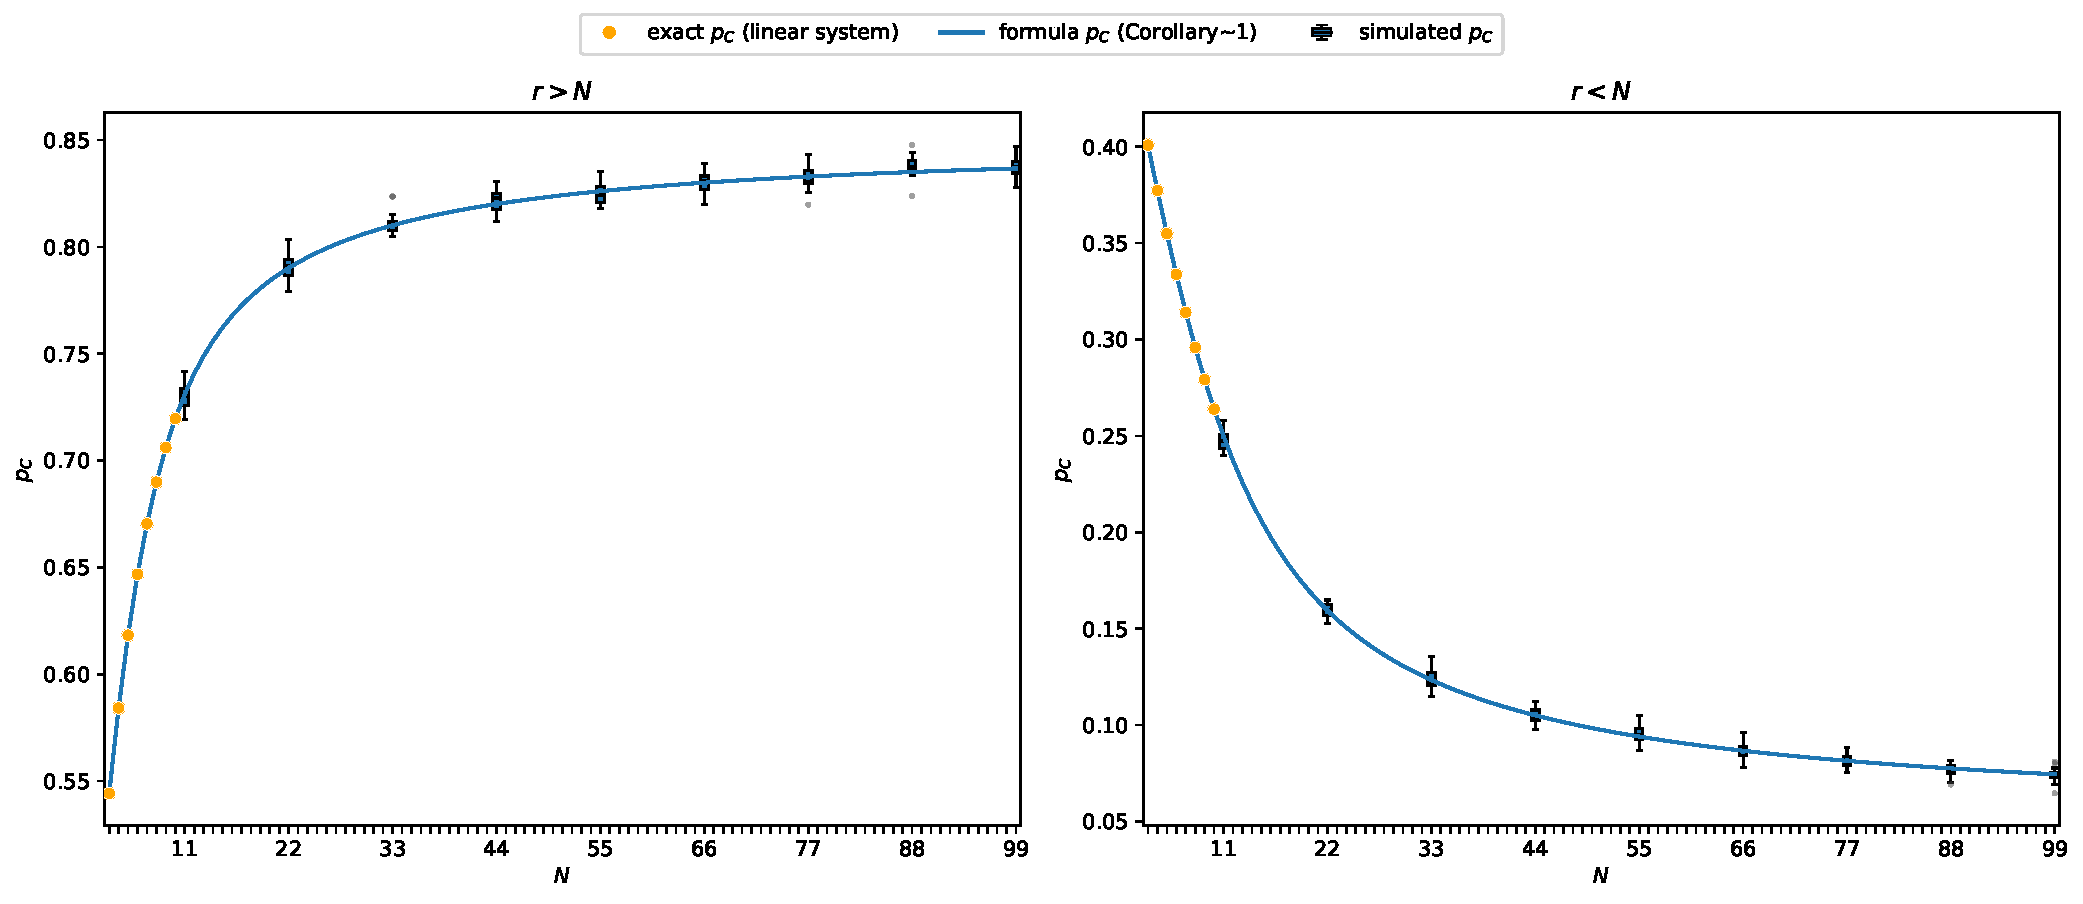
\includegraphics[width=\textwidth]{simulations.pdf}
  \caption{Validation of formula~\eqref{eq:pC} on a heterogeneous group with
    \(\alpha_i=i\), \(\beta=0.5\), \DIFdelbeginFL \DIFdelFL{\(\mu_{i0}=0.05\)}\DIFdelendFL \DIFaddbeginFL \DIFaddFL{\(\mu_{iC}=0.05\)}\DIFaddendFL , \DIFdelbeginFL \DIFdelFL{\(\mu_{i1}=0.15\)}\DIFdelendFL \DIFaddbeginFL \DIFaddFL{\(\mu_{iD}=0.15\)}\DIFaddendFL .
    \textit{Left:} \(r=2N\) (so \(r>N\) for all \(N\)).
    \textit{Right:} \(r=N/2\) (so \(r<N\) for all \(N\)).
    \DIFdelbeginFL \DIFdelFL{Orange dots: }\DIFdelendFL \DIFaddbeginFL \DIFaddFL{The }\DIFaddendFL exact \(p_C\) from the full \(2^N\) linear system (feasible only
    for small \(N\))\DIFdelbeginFL \DIFdelFL{.
    Blue curve: }\DIFdelendFL \DIFaddbeginFL \DIFaddFL{, the }\DIFaddendFL formula~\eqref{eq:pC}
    (Corollary~\ref{cor:exact-pC})\DIFdelbeginFL \DIFdelFL{.
    Blue boxes: }\DIFdelendFL \DIFaddbeginFL \DIFaddFL{, and the }\DIFaddendFL distribution of \(p_C\) across
    19 independent \DIFaddbeginFL \DIFaddFL{simulation }\DIFaddendFL runs of 5{,}000 \DIFdelbeginFL \DIFdelFL{simulation }\DIFdelendFL steps each (with the first
    500 steps discarded as warm-up; outliers shown) \DIFaddbeginFL \DIFaddFL{are in good agreement}\DIFaddendFL .
    All values \DIFaddbeginFL \DIFaddFL{were }\DIFaddendFL obtained using~\cite{harry_foster_2026_19495532}.}
  \label{fig:validation}
\end{figure}

\begin{table}[ht]
  \centering
  \begin{tabular}{lrr}
\toprule
State $\mathbf{a}$ & Formula $\pi_{\mathbf{a}}$ & Exact $\pi_{\mathbf{a}}$ \\
\midrule
DDD & 0.0367 & 0.0367 \\
DDC & 0.3299 & 0.3299 \\
DCD & 0.0367 & 0.0367 \\
DCC & 0.3299 & 0.3299 \\
CDD & 0.0133 & 0.0133 \\
CDC & 0.1201 & 0.1201 \\
CCD & 0.0133 & 0.0133 \\
CCC & 0.1201 & 0.1201 \\
\bottomrule
\end{tabular}

  \caption{Stationary-distribution probabilities \(\pi_{\mathbf{a}}\) for all
    eight states \(\mathbf{a}\in\{D,C\}^3\) with \(N=3\), \(\alpha_1=1\),
    \(\alpha_2=2\), \(\alpha_3=3\), \(\beta=2\), \DIFdelbeginFL \DIFdelFL{\(\mu_{i0}=\mu_{i1}=0.1\)}\DIFdelendFL \DIFaddbeginFL \DIFaddFL{\(\mu_{iC}=\mu_{iD}=0.1\)}\DIFaddendFL , and
    per-player multipliers
    \(r_1=1{<}N{=}r_2{=}3{<}r_3{=}9\).
    Formula: product measure~\eqref{eq:stationary} (Theorem~\ref{thm:stationary});
    Exact: values from the \(2^N\) linear system obtained
    using~\cite{harry_foster_2026_19495532}.
    Both columns \DIFaddbeginFL \DIFaddFL{are given }\DIFaddendFL to four decimal places.}
  \label{tab:stationary}
\end{table}

We now specialise the structural consequences of Section~\ref{sec:consequences} to the
public goods game, where \(\delta_i=\alpha_i(1-r_i/N)\) makes every quantity explicit in
the group size and the players' own parameters.

\DIFaddbegin \DIFadd{At \(\beta_i=0\) the payoff parameters drop out
(Remark~\ref{rem:neutral}); the left panel of Figure~\ref{fig:panel} shows the
curves \(p_i(\beta_i)\) converging to \(p_i=\tfrac{1}{2}\) at \(\beta_i=0\)
before diverging in the direction set by \(r_i\) relative to \(N\).
}

\DIFaddend For the PGG, \(\delta_i<0\) precisely when \(r_i>N\), so
the symmetric-mutation threshold of Corollary~\ref{cor:threshold} becomes \(r_i>N\): a
player cooperates the majority of the time exactly when their personal multiplier on the
public good exceeds the group size, that is, when they \DIFdelbegin \DIFdel{extract more from the pool per unit
contributed than they put in}\DIFdelend \DIFaddbegin \DIFadd{are a net beneficiary}\DIFaddend .
Without mutation this is the cooperation-dominance condition
of~\cite{couto2023multiplayer} (their \(c_i<b_i/N\)). The centre panel of
Figure~\ref{fig:panel} illustrates this, with curves at \DIFdelbegin \DIFdel{\(r>N\) }\DIFdelend \DIFaddbegin \DIFadd{\(r_i>N\) }\DIFaddend lying above
\(p_i=\tfrac{1}{2}\) and curves at \DIFdelbegin \DIFdel{\(r<N\) }\DIFdelend \DIFaddbegin \DIFadd{\(r_i<N\) }\DIFaddend lying below it. Since the comparison is
between \(r_i\) and \(N\), a player with a fixed multiplier becomes a \DIFdelbegin \DIFdel{non-benefactor }\DIFdelend \DIFaddbegin \DIFadd{net contributor
}\DIFaddend once the group \DIFaddbegin \DIFadd{size }\DIFaddend exceeds \(r_i\): cooperation in large groups therefore requires
multipliers that grow with \(N\). For a \DIFdelbegin \DIFdel{non-beneficiary }\DIFdelend \DIFaddbegin \DIFadd{net contributor }\DIFaddend (\(r_i<N\), so
\(\delta_i>0\)) a cooperative mutation bias \DIFdelbegin \DIFdel{\(\mu_{i0}>\mu_{i1}\) }\DIFdelend \DIFaddbegin \DIFadd{\(\mu_{iC}>\mu_{iD}\) }\DIFaddend can still raise
\(p_i\) above \(\tfrac{1}{2}\), as in Corollary~\ref{cor:threshold}.

\DIFdelbegin \DIFdel{At \(\beta_i=0\) the payoff parameters drop out
(Remark~\ref{rem:neutral}); the right panel of Figure~\ref{fig:panel} shows
\(p_i=\tfrac{1}{2}\) for every \(\alpha_i\) and \(r_i\), and the left panel shows the
curves converging to \(p_i=\tfrac{1}{2}\) at \(\beta_i=0\) before diverging in the
direction set by \(r_i\) relative to \(N\).
}%DIFDELCMD < 

%DIFDELCMD < \begin{figure}[ht]
%DIFDELCMD <   \centering
%DIFDELCMD <   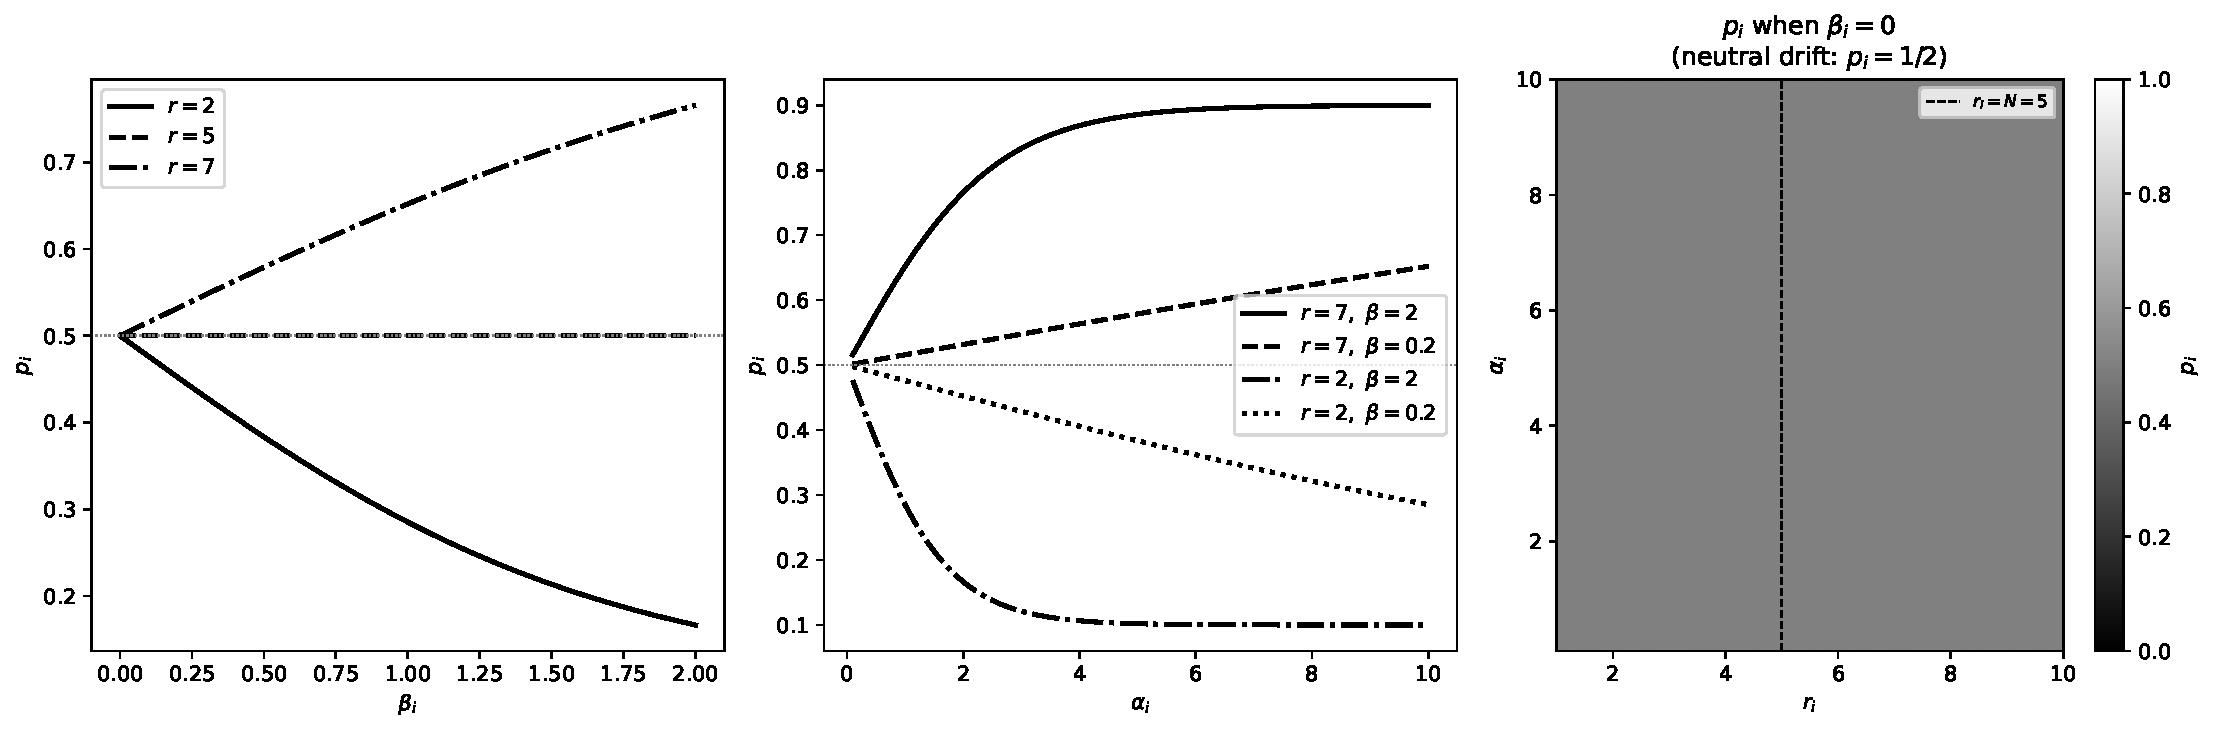
\includegraphics[width=\textwidth]{big_panel.pdf}
%DIFDELCMD <   %%%
%DIFDELCMD < \caption{%
{%DIFAUXCMD
\DIFdelFL{Structural properties of \(p_i\) for a single player with \(N = 5\),
    \(\mu_{i0} = \mu_{i1} = 0.1\).
    }\textit{\DIFdelFL{Left:}} %DIFAUXCMD
\DIFdelFL{\(p_i\) as a function of \(\beta_i\) (\(\alpha_i = 2\))
    for \(r_i < N\), \(r_i = N\), and \(r_i > N\); all curves pass through
    \(p_i = \tfrac{1}{2}\) at \(\beta_i = 0\) (Remark~\ref{rem:neutral}).
    }\textit{\DIFdelFL{Centre:}} %DIFAUXCMD
\DIFdelFL{\(p_i\) as a function of \(\alpha_i\) for two values of
    \(r_i\) and \(\beta_i\); curves above (below) \(\tfrac{1}{2}\) correspond
    to \(r_i > N\) (\(r_i < N\)).
    }\textit{\DIFdelFL{Right:}} %DIFAUXCMD
\DIFdelFL{\(p_i(\alpha_i, r_i)\) at \(\beta_i = 0\), confirming
    \(p_i = \tfrac{1}{2}\) everywhere (Remark~\ref{rem:neutral}); the dashed
    line marks \(r_i = N\).}}
  %DIFAUXCMD
%DIFDELCMD < \label{fig:panel}
%DIFDELCMD < \end{figure}
%DIFDELCMD < 

%DIFDELCMD < %%%
\DIFdelend For the PGG, \(\phi_i(\delta_i)>\tfrac{1}{2}\iff r_i>N\), so the sign of
\(\partial\pC/\partial\mu\) in Proposition~\ref{prop:balance} is set by
whether \DIFdelbegin \DIFdel{the group is}\DIFdelend \DIFaddbegin \DIFadd{players are}\DIFaddend , on average, \DIFaddbegin \DIFadd{net }\DIFaddend beneficiaries: common mutation raises
aggregate cooperation when most players have \(r_i<N\) and lowers it when most have
\(r_i>N\). \DIFaddbegin \DIFadd{The right panel of Figure~\ref{fig:panel} shows this mutation-selection
balance for a single player: \(p_i\) is affine in the symmetric mutation rate \(\mu\)
(Proposition~\ref{prop:balance}), interpolating between the mutation-free value
\(\phi_i(\delta_i)\) at \(\mu=0\) and \(\tfrac{1}{2}\) at \(\mu=\tfrac{1}{2}\),
increasing in \(\mu\) for a net contributor and decreasing for a net beneficiary.
}\DIFaddend 

\DIFaddbegin \begin{figure}[!htbp]
  \centering
  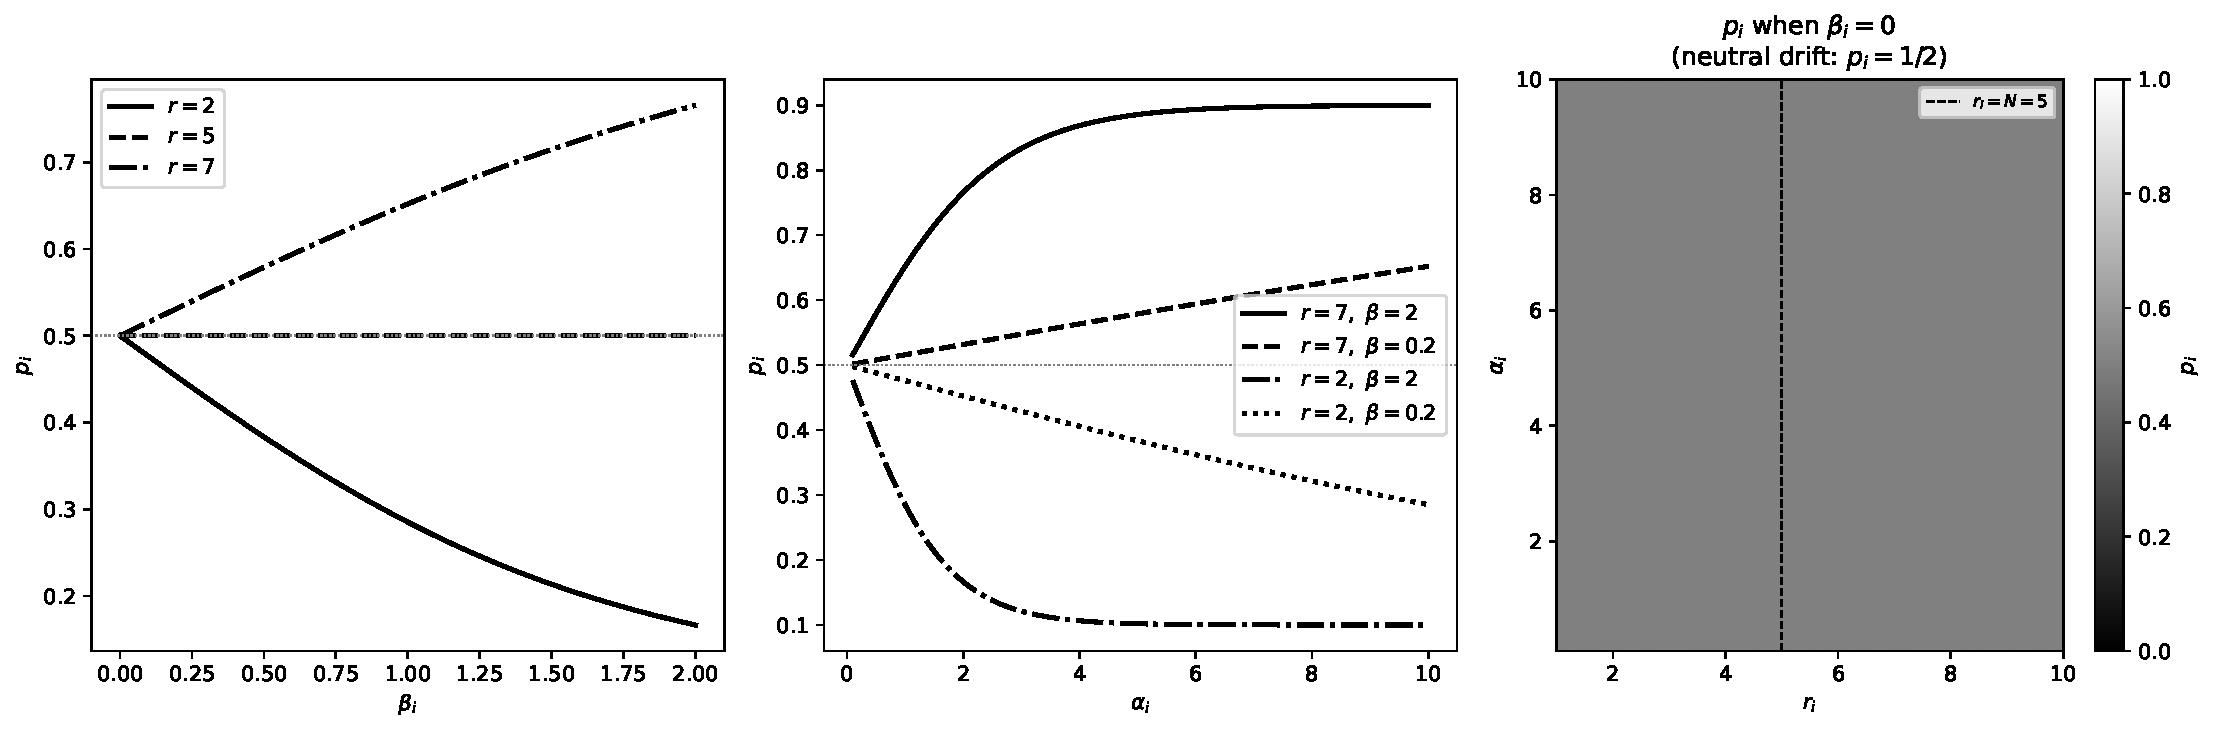
\includegraphics[width=\textwidth]{big_panel.pdf}
  \caption{\DIFaddFL{Structural properties of \(p_i\) for a single player with \(N = 5\)
    and, unless varied, symmetric mutation \(\mu_{iC} = \mu_{iD} = 0.1\).
    }\textit{\DIFaddFL{Left:}} \DIFaddFL{\(p_i\) as a function of \(\beta_i\) (\(\alpha_i = 2\))
    for \(r_i < N\), \(r_i = N\), and \(r_i > N\); all curves pass through
    \(p_i = \tfrac{1}{2}\) at \(\beta_i = 0\) (Remark~\ref{rem:neutral}).
    }\textit{\DIFaddFL{Centre:}} \DIFaddFL{\(p_i\) as a function of \(\alpha_i\) for two values of
    \(r_i\) and \(\beta_i\); curves above (below) \(\tfrac{1}{2}\) correspond
    to \(r_i > N\) (\(r_i < N\)).
    }\textit{\DIFaddFL{Right:}} \DIFaddFL{\(p_i\) as a function of the symmetric mutation rate
    \(\mu_{iC} = \mu_{iD} = \mu\) (\(\alpha_i = 2\), \(\beta_i = 2\)) for
    \(r_i < N\), \(r_i = N\), and \(r_i > N\); each line is affine in \(\mu\)
    (Proposition~\ref{prop:balance}) and reaches \(p_i = \tfrac{1}{2}\) at
    \(\mu = \tfrac{1}{2}\).}}
  \label{fig:panel}
\end{figure}

\DIFaddend Figure~\ref{fig:mutation} isolates the
role of mutation for a single player. A larger selection intensity \(\beta_i\) makes the
player respond more sharply to payoff differences, adopting the higher-payoff action
with
greater probability, whereas \(\beta_i=0\) is payoff-blind random choice. Without
mutation
\(p_i\) is driven to \(0\) or \(1\) as \(\beta_i\) grows, whereas mutation confines
\(p_i\) to \DIFdelbegin \DIFdel{\([\mu_{i0},1-\mu_{i1}]\) }\DIFdelend \DIFaddbegin \DIFadd{\([\mu_{iC},1-\mu_{iD}]\) }\DIFaddend (Proposition~\ref{prop:strong}). The two
panels show
the same player (\(r_i=7\), \(\alpha_i=2\)) at \(N=5\) and \(N=200\): increasing the
group
size alone turns the \DIFdelbegin \DIFdel{benefactor }\DIFdelend \DIFaddbegin \DIFadd{net beneficiary }\DIFaddend (\(r_i>N\), \(p_i\) rising to \(1-\mu\)) into a
\DIFdelbegin \DIFdel{non-benefactor }\DIFdelend \DIFaddbegin \DIFadd{net contributor }\DIFaddend (\(r_i<N\), \(p_i\) falling to \(\mu\)).

\DIFdelbegin %DIFDELCMD < \begin{figure}[ht]
%DIFDELCMD <   %%%
\DIFdelendFL \DIFaddbeginFL \begin{figure}[!htbp]
  \DIFaddendFL \centering
  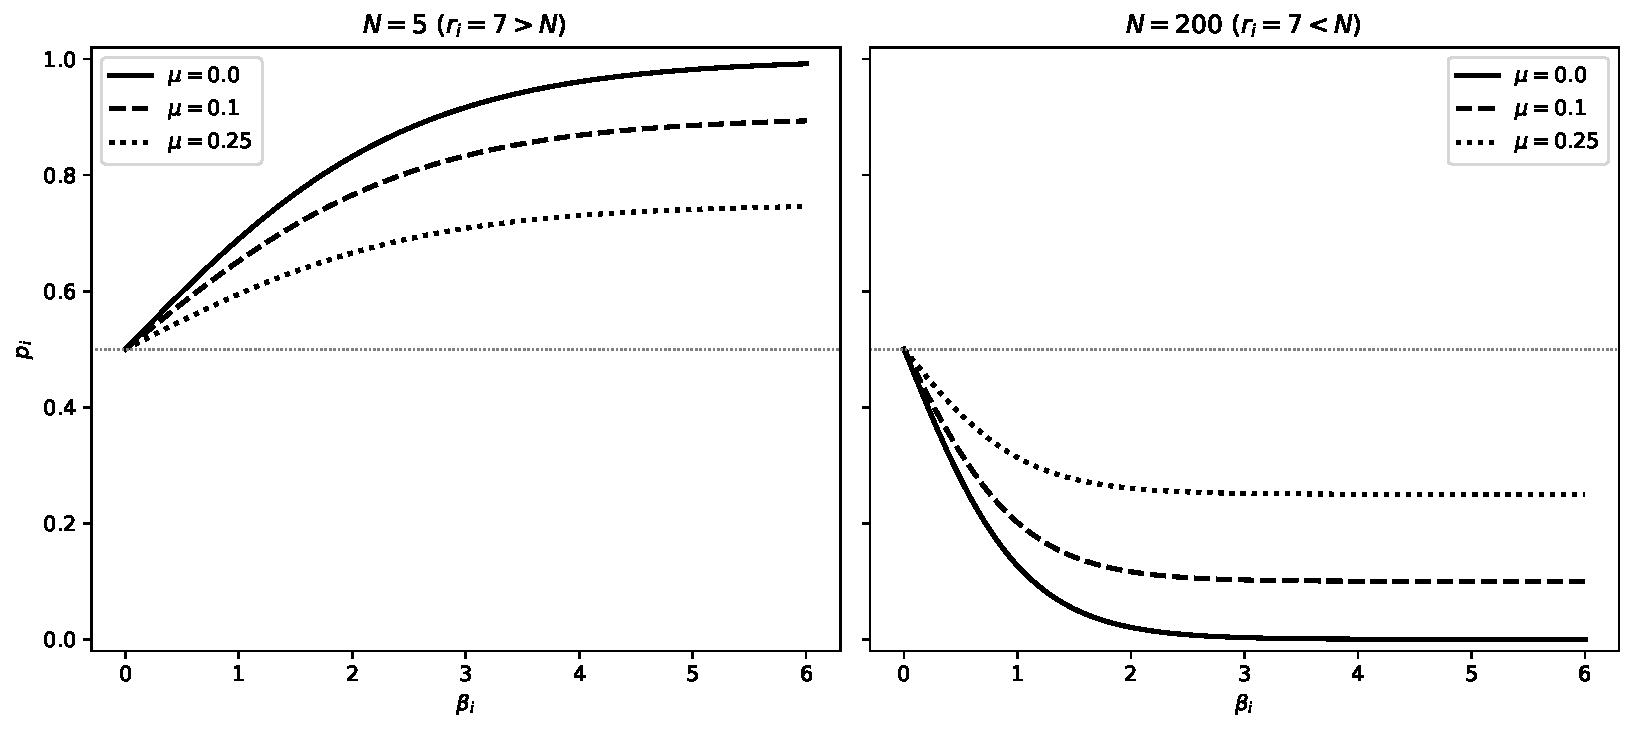
\includegraphics[width=\textwidth]{mutation.pdf}
  \caption{Effect of mutation on the cooperation probability of a single player with
    multiplier \(r_i=7\) and contribution \(\alpha_i=2\), as a function of the selection
    intensity \(\beta_i\) for symmetric mutation \(\mu\in\{0,0.1,0.25\}\), at two group
    sizes.
    \textit{Left:} \(N=5\), so \(r_i>N\) and the player is a \DIFdelbeginFL \DIFdelFL{benefactor}\DIFdelendFL \DIFaddbeginFL \DIFaddFL{net beneficiary}\DIFaddendFL ; \(p_i\)
    rises towards \(1-\mu\) as \(\beta_i\) grows.
    \textit{Right:} \(N=200\), so the same player now has \(r_i<N\) and is a
    \DIFdelbeginFL \DIFdelFL{non-benefactor}\DIFdelendFL \DIFaddbeginFL \DIFaddFL{net contributor}\DIFaddendFL ; \(p_i\) falls towards \(\mu\).
    In both panels the \(\mu=0\) curve is the mutation-free dynamics
    of~\cite{couto2023multiplayer}, reaching \(1\) or \(0\); mutation confines \(p_i\)
to
    \([\mu,1-\mu]\). \DIFaddbeginFL \DIFaddFL{The alternative mutation scheme of
    Section~\ref{sec:alternative-mutation} with rate \(\nu=\mu/(1-\mu)\) is
    also shown for \(\mu\in\{0.1,0.25\}\); as established by
    Proposition~\ref{prop:equivalence}, it coincides with the corresponding
    curve. }\DIFaddendFL Increasing the group size alone turns the \DIFdelbeginFL \DIFdelFL{benefactor }\DIFdelendFL \DIFaddbeginFL \DIFaddFL{net beneficiary }\DIFaddendFL into a
    \DIFdelbeginFL \DIFdelFL{non-benefactor}\DIFdelendFL \DIFaddbeginFL \DIFaddFL{net contributor}\DIFaddendFL .}
  \label{fig:mutation}
\end{figure}

\begin{remark}[Role of heterogeneity]\label{rem:heterogeneity}

For the PGG with \(r_i\neq N\), both \(\partial p_i/\partial\alpha_i\) and
\(\partial p_i/\partial\beta_i\) are positive when \(r_i>N\) and negative when
\(r_i<N\):
each derivative carries the factor \((1-r_i/N)\) \DIFdelbegin \DIFdel{multiplied by the negative quantity
\(\phi_i'\)}\DIFdelend \DIFaddbegin \DIFadd{together with a negative sign
stemming from the derivative \(\phi_i'<0\)}\DIFaddend , so its sign is that of \(r_i/N-1\).
Indeed, \(\beta_i\) and \(\alpha_i\) enter
\(p_i\) only through the product \(\beta_i\alpha_i\), so a change in selection intensity
has
the same effect as a proportional change in contribution. Under symmetric mutation,
raising
the mutation rate instead pulls \(p_i\) towards \(\tfrac{1}{2}\), lowering cooperation
when
\(r_i>N\) and raising it when \(r_i<N\); with asymmetric mutation \(p_i\) is pulled
towards
its neutral value \DIFdelbegin \DIFdel{\((1+\mu_{i0}-\mu_{i1})/2\)}\DIFdelend \DIFaddbegin \DIFadd{\((1+\mu_{iC}-\mu_{iD})/2\)}\DIFaddend .

\end{remark}

A \DIFdelbegin \DIFdel{player who benefits from the public good }\DIFdelend \DIFaddbegin \DIFadd{net beneficiary }\DIFaddend (\(r_i>N\)) cooperates more as they contribute more or
respond more strongly to payoff differences; a \DIFdelbegin \DIFdel{non-benefactor }\DIFdelend \DIFaddbegin \DIFadd{net contributor }\DIFaddend (\(r_i<N\))
does the opposite. Each player's long-run cooperation is thus determined entirely by
their own
\DIFdelbegin \DIFdel{\((\alpha_i,\beta_i,r_i,\mu_{i0},\mu_{i1})\) }\DIFdelend \DIFaddbegin \DIFadd{\((\alpha_i,\beta_i,r_i,\mu_{iC},\mu_{iD})\) }\DIFaddend and the group size \(N\); the other
players'
parameters do not enter.

\DIFaddbegin \section{\DIFadd{Non-additive games}}\label{sec:non-additive}

\DIFadd{The results so far rely on additivity. When \(\Delta f_i(\bfa;b)\) depends on
\(\bfa_{-i}\), the kernel \(K_i\) is not defined, the players' actions are
coupled, and the stationary distribution must be computed from the full
\(\prod_i L_i\) linear system. In this section we explore numerically how
mutation behaves in that setting, taking the non-linear public goods game as
a case study.
}

\DIFadd{In the non-linear PGG the pool is no longer proportional to the total
contribution \(X(\bfa)=\sum_j \alpha_j a_j\): each unit contributed changes
the marginal value of the next by a factor \(w>0\), so that the payoff to
player \(i\) is
}\begin{equation}\DIFadd{\label{eq:nonlinear-payoff}
  f_i(\bfa) = \frac{r}{N}\,\frac{w^{X(\bfa)}-1}{w-1} - \alpha_i a_i,
}\end{equation}
\DIFadd{with the linear game~\eqref{eq:payoff} with common multiplier \(r_i=r\)
recovered in the limit \(w\to1\). For unit contributions (\(\alpha_i=1\))
the pool is \((r/N)(1+w+\cdots+w^{k-1})\) with \(k=\sum_j a_j\) cooperators:
this is the synergy and discounting game of~\mbox{%DIFAUXCMD
\cite{hauert2006synergy}}\hskip0pt%DIFAUXCMD
, in
which the \(j\)-th contribution is worth a factor \(w\) of the
\((j-1)\)-th. For \(w>1\) each additional contribution is worth more than
the last: the benefits of cooperation are }\emph{\DIFadd{synergistically enhanced}}\DIFadd{,
as when collaborators complement one another. For \(w<1\) they are
}\emph{\DIFadd{discounted}}\DIFadd{, as when the public good saturates and further
contributions bring diminishing returns. With unit contributions, switching
player \(i\) to cooperation adds \((r/N)\,w^{k_{-i}}\) to their share of the
pool, where \(k_{-i}\) is the number of co-operating co-players, so
cooperation is individually favoured precisely when
\((r/N)\,w^{k_{-i}}>1\). For \(w=1\) this is the additive condition \(r>N\)
of Section~\ref{sec:payoff}; for \(w\neq1\) the incentive depends on the
co-players and the game is not additive. With discounting (\(w<1\))
cooperation is favoured only when few others cooperate; with synergy
(\(w>1\)) only when enough others do.
}

\DIFadd{Figure~\ref{fig:non-additive} reports exact quantities computed from the
full \(2^N\) linear system using~\mbox{%DIFAUXCMD
\cite{harry_foster_2026_19495532}}\hskip0pt%DIFAUXCMD
, for
\(N=8\). The top row takes unit contributions; the top-left and top-centre
panels take \(r=4\),
so that \(r<N\) and defection dominates the linear game. Three observations
follow. First, the \(w=1\) values coincide with the closed form of
Corollary~\ref{cor:exact-pC} and the affine balance of
Proposition~\ref{prop:balance}, a numerical check of the additive theory.
Second, with discounting the additive pattern persists qualitatively:
cooperation is low, mutation raises it towards the neutral level
\(\tfrac{1}{2}\), and \(p_C\) is no longer exactly affine in \(\mu\). Third,
with synergy the behaviour changes altogether: cooperation is nearly full at
weak mutation, and mutation lowers it towards \(\tfrac{1}{2}\).
}

\DIFadd{The synergy case shows that mutation can produce high cooperation where none
is expected. At \(w=1.4\) the game is bistable: all-defect and all-cooperate
are both strict equilibria, since the first cooperator loses
\(1-r/N>0\) regardless of \(w\), whilst a defector in a fully
cooperative group forgoes \((r/N)w^{N-1}-1>0\). In the
strong-selection limit the mutation-free dynamics therefore remain at
whichever equilibrium the initial state reaches: started from defection, no
cooperation ever arises. Any positive mutation rate makes the chain ergodic,
and the top-centre panel of Figure~\ref{fig:non-additive} shows the outcome.
For \(w\le1\) strong selection drives cooperation down to the mutation floor
\(\mu\) (Proposition~\ref{prop:strong} for \(w=1\)); for \(w=1.4\)
increasing the selection intensity instead drives \(p_C\) up, towards
approximately \(1-\mu\). Occasional payoff-independent switches allow the
group to escape the all-defect equilibrium; once at least three co-players
cooperate (\((r/N)w^{k}>1\) for \(k\ge3\) at these parameters),
introspection favours joining them, and the group is carried to full
cooperation. Mutation therefore acts as an equilibrium-selection device in
non-additive games, echoing the role of rare mutations in stochastic
evolutionary dynamics~\mbox{%DIFAUXCMD
\cite{fudenberg2006evolutionary}}\hskip0pt%DIFAUXCMD
.
}

\DIFadd{Beyond additivity there can also be an optimal, strictly positive mutation
rate. For additive games Proposition~\ref{prop:balance} rules this out:
under common symmetric mutation, aggregate cooperation is affine and hence
monotone in \(\mu\). The top-right panel of Figure~\ref{fig:non-additive}
shows a smaller multiplier with stronger synergy (\(r=2\), \(w=1.5\)), for
which cooperation is individually favoured only once four co-players
cooperate. At \(\beta=5\) cooperation is nearly full at weak mutation and
noise only erodes it. At \(\beta=10\) and \(\beta=20\) the curve is no
longer monotone: \(p_C\) peaks at \(\mu^*\approx0.02\) and
\(\mu^*\approx0.03\) respectively, with the peak falling as selection
strengthens. A moderate amount of noise maximises cooperation: enough
mutation to seed the escape from the all-defect equilibrium, but not so much
as to erode the cooperative one.
}

\DIFadd{Additivity is also precisely the point at which the players' actions
decouple. The bottom row of Figure~\ref{fig:non-additive} shows the pairwise
correlations \(\mathrm{corr}(a_i,a_j)\) under the stationary distribution
for the heterogeneous group of Figure~\ref{fig:validation} (contributions
\(\alpha_i=i\), \(\beta=0.5\)), here with \(r=4\) and symmetric mutation
\(\mu=0.05\); since the total contribution reaches \(36\), mild synergy and
discounting (\(w=1.05\) and \(w=0.95\)) suffice. For \(w=1\) every pairwise
correlation is zero, as the product measure of Theorem~\ref{thm:general}
requires, despite the heterogeneity. For \(w=0.95\) all pairs are weakly
negatively correlated: under discounting a player's incentive to cooperate
falls with the contributions of co-operating co-players, favouring
anti-coordination. For \(w=1.05\), where the two strict equilibria compete,
the correlations are positive and substantial, and increase with both
players' contributions: the two largest contributors are the most strongly
coupled (\(\mathrm{corr}(a_7,a_8)\approx0.35\)). Beyond additivity a
player's long-run behaviour is thus tied to their co-players' parameters, in
contrast to the additive case, where it depends only on their own; raising
the mutation rate erodes every off-diagonal correlation towards zero.
}

\begin{figure}[!htbp]
  \centering
  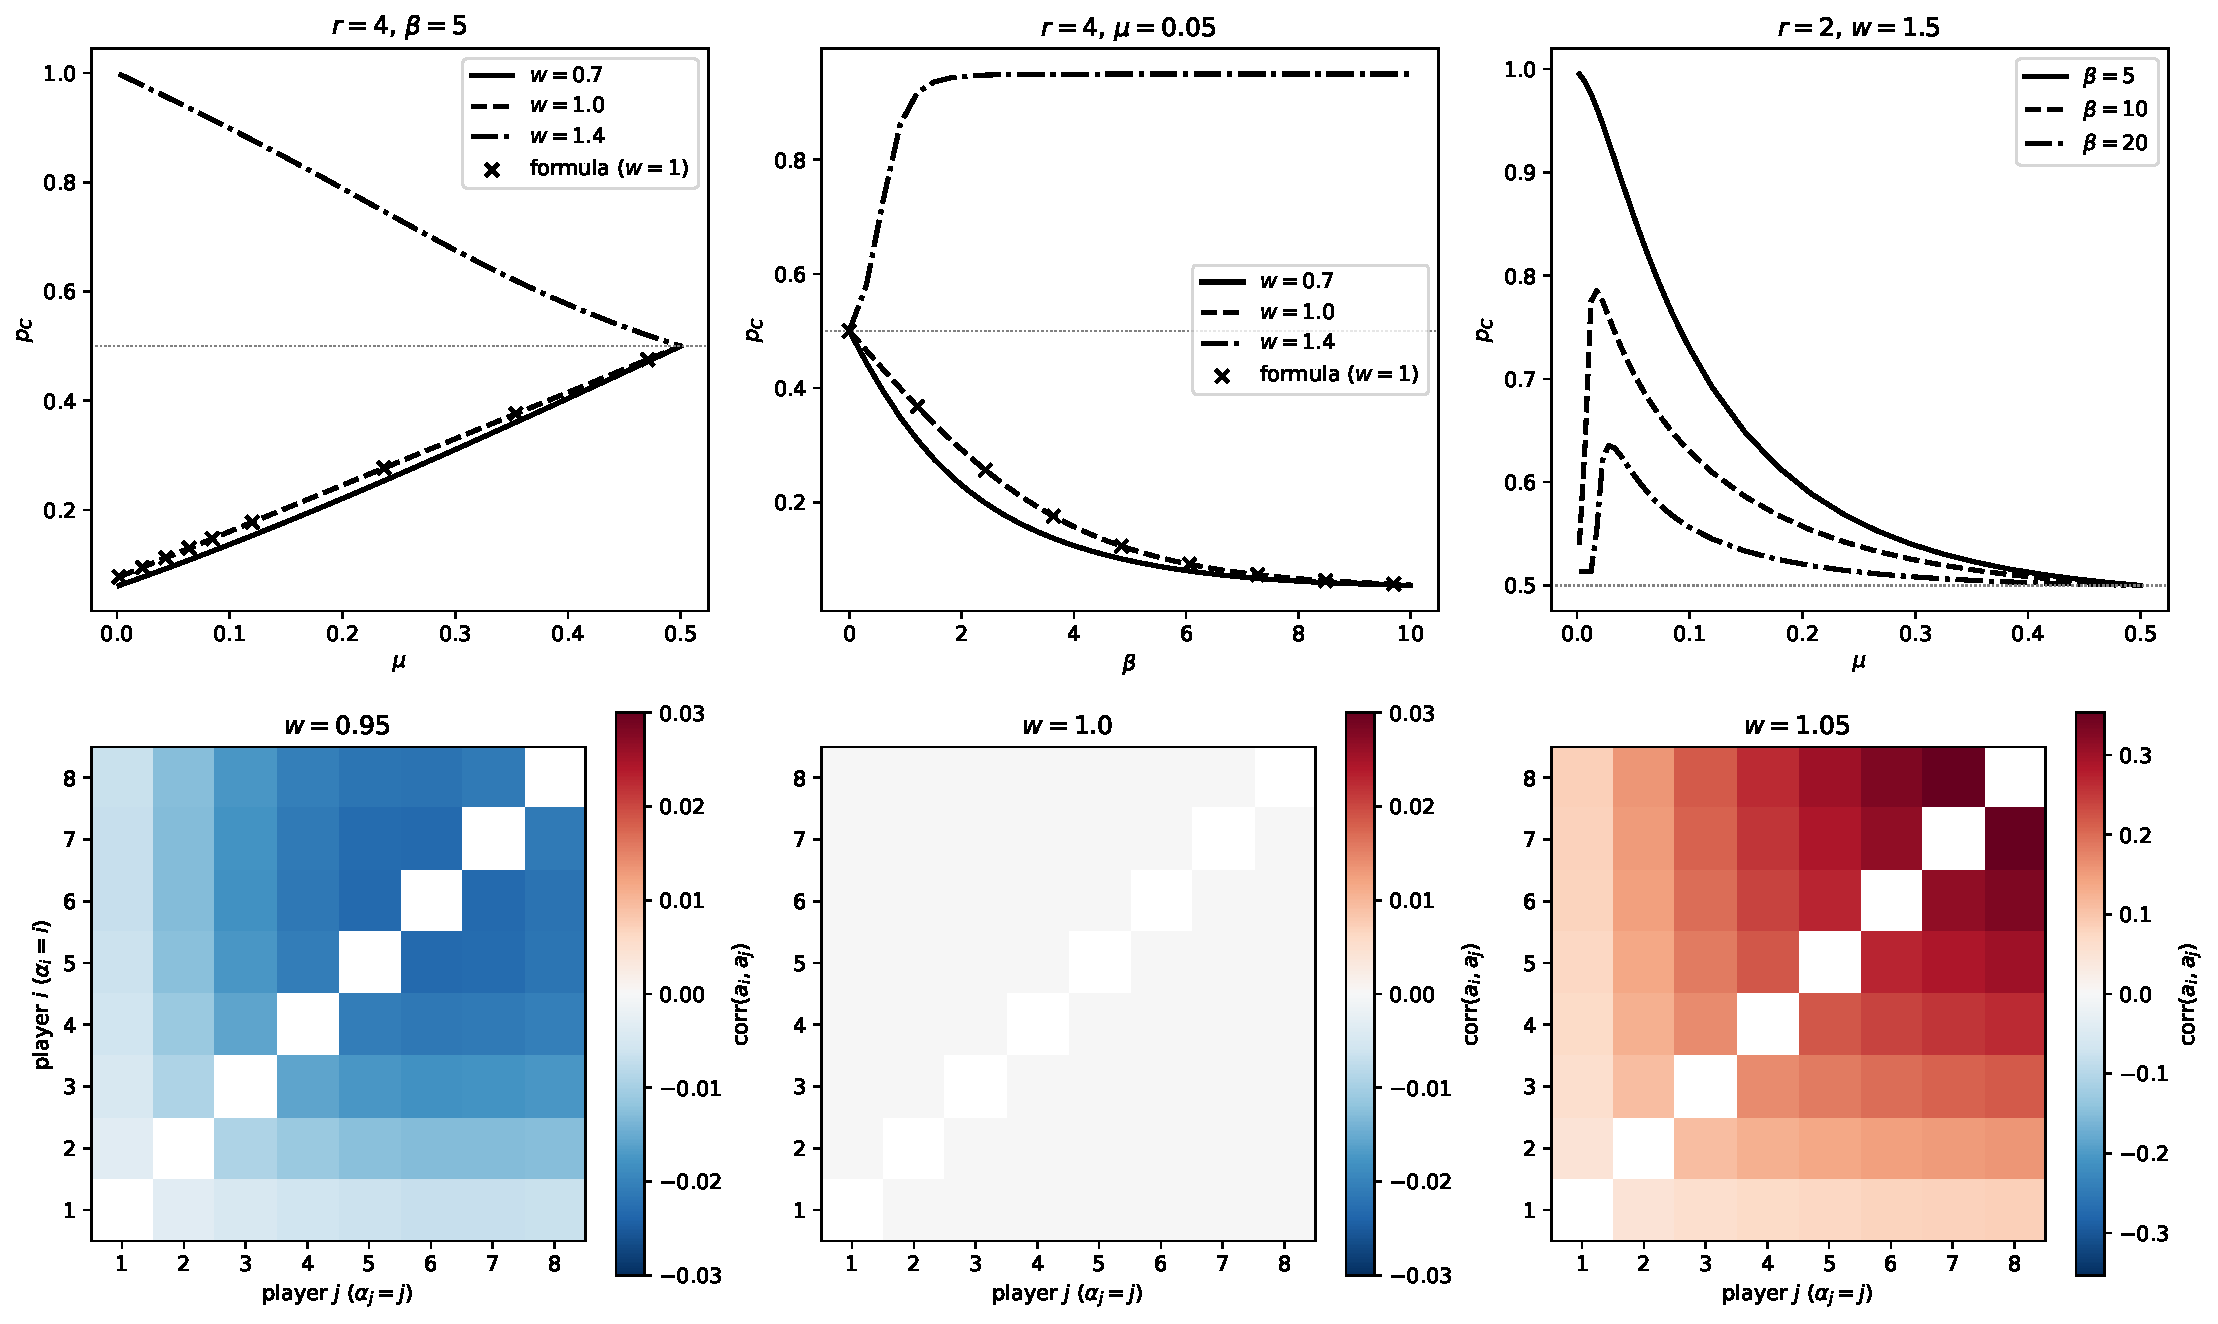
\includegraphics[width=\textwidth]{non_additive.pdf}
  \caption{\DIFaddFL{Mutation in the non-linear public goods
    game~\eqref{eq:nonlinear-payoff} with \(N=8\); the top row takes unit
    contributions (\(\alpha_i=1\)). All
    values were computed exactly from the full \(2^N\) linear system
    using~\mbox{%DIFAUXCMD
\cite{harry_foster_2026_19495532}}\hskip0pt%DIFAUXCMD
.
    }\textit{\DIFaddFL{Top left:}} \DIFaddFL{\(p_C\) as a function of the common symmetric
    mutation rate \(\mu\) at \(r=4\), \(\beta=5\), for discounting
    (\(w=0.7\)), the linear game (\(w=1\)), and synergy (\(w=1.4\)); the
    closed form of Corollary~\ref{cor:exact-pC} matches the \(w=1\) values
    well. The \(w=0.7\) curve follows the additive pattern
    but is no longer affine, whilst the \(w=1.4\) curve starts near full
    cooperation and falls towards \(\tfrac{1}{2}\).
    }\textit{\DIFaddFL{Top centre:}} \DIFaddFL{\(p_C\) as a function of \(\beta\) at \(r=4\),
    \(\mu=0.05\). For \(w\le1\) strong selection drives cooperation to the
    mutation floor \(\mu\); for \(w=1.4\) it selects the cooperative
    equilibrium and \(p_C\) approaches \(1-\mu\).
    }\textit{\DIFaddFL{Top right:}} \DIFaddFL{\(p_C\) as a function of \(\mu\) for a bistable
    synergy game (\(r=2\), \(w=1.5\)). At \(\beta=10\) and \(\beta=20\)
    cooperation is maximised at a strictly positive mutation rate, which
    Proposition~\ref{prop:balance} rules out for additive games.
    }\textit{\DIFaddFL{Bottom row:}} \DIFaddFL{pairwise correlations \(\mathrm{corr}(a_i, a_j)\)
    under the stationary distribution for the heterogeneous group of
    Figure~\ref{fig:validation} (contributions \(\alpha_i=i\),
    \(\beta=0.5\)), at \(r=4\) and \(\mu=0.05\). The axes give the player
    indices \(i\) and \(j\), which, since \(\alpha_i=i\), also order the
    players by contribution; diagonals are omitted and the colour scales
    differ between panels. For \(w=1\) every entry is
    zero (Theorem~\ref{thm:general}); for \(w=0.95\) all pairs are weakly
    negatively correlated; for \(w=1.05\) the correlations are positive and
    increase with both players' contributions.}}
  \label{fig:non-additive}
\end{figure}

\DIFaddend \section{Conclusion}\label{sec:conclusion}

Building on the additive-game results of~\cite{couto2023multiplayer}, we have shown that
introspection dynamics with mutation on any additive game remains exactly
solvable\DIFdelbegin \DIFdel{. When
\(\Delta f_i\) depends only on \(a_i\), each selection of player \(i\) places them in state
\(C\) with probability \(p_i\) regardless of current state (Theorem~\ref{thm:decomp}), and
}\DIFdelend \DIFaddbegin \DIFadd{: in the long run the players behave independently, so }\DIFaddend the
stationary distribution is a product measure\DIFaddbegin \DIFadd{, for any finite number of
actions per player }\DIFaddend (Theorem~\DIFdelbegin \DIFdel{\ref{thm:stationary}); the
}\DIFdelend \DIFaddbegin \DIFadd{\ref{thm:general}), and its computation reduces
to one small linear system per player. The }\DIFaddend product-measure structure, due
to~\cite{couto2023multiplayer} for the no-mutation case, is \DIFaddbegin \DIFadd{thus }\DIFaddend preserved
under mutation. For \DIFdelbegin \DIFdel{the }\DIFdelend \DIFaddbegin \DIFadd{two actions, additivity makes each player's choice
forgetful: whenever a player is selected they cooperate with a fixed
probability, determined by their own payoff difference, selection intensity,
and mutation probabilities alone (Theorem~\ref{thm:decomp}), and the
stationary distribution is fully explicit (Theorem~\ref{thm:stationary}),
although this closed form is special to two actions. For the }\DIFaddend heterogeneous
public goods game, the linear payoff structure implies additivity
(Lemma~\ref{lem:payoff-identity}), and the long-run cooperation probability has a closed
form with \(N\) terms rather than \(2^N\) (Corollary~\ref{cor:exact-pC}).

The \DIFdelbegin \DIFdel{approach }\DIFdelend \DIFaddbegin \DIFadd{exact analysis }\DIFaddend does not extend to games that are not additive\DIFdelbegin \DIFdel{. When
\(\Delta f_i(\bfa)\) depends on \(\bfa_{-i}\), the
per-player chains are coupledand
}\DIFdelend \DIFaddbegin \DIFadd{: when the
payoff difference a player evaluates depends on }\DIFaddend the \DIFaddbegin \DIFadd{co-players' actions, the
players' behaviours are coupled, the }\DIFaddend stationary distribution is no longer a
product measure\DIFdelbegin \DIFdel{; }\DIFdelend \DIFaddbegin \DIFadd{, and }\DIFaddend the full \(2^N\) linear system must be solved in
general. Games such as the Stag Hunt \DIFdelbegin \DIFdel{(\(M_2\) of
(\ref{eq:games_from_couto_2022})) }\DIFdelend contain payoff cross terms \DIFdelbegin \DIFdel{\(a_i a_{-i}\) }\DIFdelend that cannot
be eliminated by rescaling, so no reformulation brings them within the scope
of the \DIFdelbegin \DIFdel{present results. }\DIFdelend \DIFaddbegin \DIFadd{closed forms. Our numerical exploration of the non-linear public
goods game (Section~\ref{sec:non-additive}) shows that mutation then takes
on further roles: it selects among coexisting strict equilibria, cooperation
can be maximised at a strictly positive mutation rate, and the players'
actions become correlated. Characterising this behaviour analytically
remains open.
}\DIFaddend 

The source code, figures, and data for this paper are under version control
and available at~\cite{foster2026repo}, in line with best practices for
research software~\cite{wilson2017good}.

\section{Acknowledgements}
We thank Marta C. Couto and Saptarshi Pal for pointing out that the product-measure
decomposition for additive games was already established in~\cite{couto2023multiplayer},
which an earlier version of this paper had failed to acknowledge\DIFaddbegin \DIFadd{. We also
thank two anonymous reviewers for their careful and constructive reports,
which led to substantial improvements throughout the paper}\DIFaddend .
Harry Foster's research was supported by EPSRC grant EP/Z535126/1.

\bibliographystyle{plain}
\bibliography{bibliography}

\end{document}
